\documentclass{article}

%%%%%%%%%%%%%%%%%%%%%%%%%%%%%%%%%%%%%%%%%%%%%%%%%%%%%%%%
% Packages
%%%%%%%%%%%%%%%%%%%%%%%%%%%%%%%%%%%%%%%%%%%%%%%%%%%%%%%%

%\usepackage[utf8]{inputenc} % for overleaf/PLM
\usepackage[latin1]{inputenc} % averil local
\usepackage[T1]{fontenc} % hyphenation
\usepackage{fullpage} % DO NOT USE IN BEAMER
\usepackage[british,UKenglish,USenglish,american]{babel}
%\usepackage{appendix}
\usepackage{amssymb,amsmath,amsthm,enumerate}
\usepackage{mathtools} % coloneqq
%\usepackage{easybmat}
\usepackage{enumitem}
%\usepackage{tikz}
%\usepackage{caption}
\usepackage{float} % [H]
%\usepackage{bbold}
\usepackage{xcolor}
\usepackage{stmaryrd} % ll/rr brackets
%\usepackage[notcite, notref]{showkeys}
%\usepackage[tworuled,vlined,nofillcomment]{algorithm2e}
\usepackage[ruled,vlined]{algorithm2e}
%\usepackage{cases} % numbered lines in cases (numcases and subnumcases)
\usepackage[overload]{empheq} % source : https://tex.stackexchange.com/questions/31951/separate-labels-in-cases
\usepackage{caption} % to have subfigures
\usepackage{subcaption} % to have subfigures
\usepackage[allcolors=teal,colorlinks]{hyperref}
\usepackage{cleveref} % \cref. 
%%%%%%%%%%%%%%%%%%%%%%%%%%%%%%%%%%%%%%%%%%%%%%%%%%%%%%%%
% Format
%%%%%%%%%%%%%%%%%%%%%%%%%%%%%%%%%%%%%%%%%%%%%%%%%%%%%%%%

\title{Numerical simulations of plasma sheaths}
\author{
	Valentin Ayot\footnote{Institut de Math\'ematiques, CNRS, UMR 5251, Universit\'e de Bordeaux, F-33405 Talence, France. \texttt{valentin.ayot@u-bordeaux.fr}}, 
	\ Mehdi Badsi\footnote{Nantes Universit\'e, Laboratoire de Math\'ematiques Jean Leray, 2 Chemin de la Houssini\`ere BP 92208, 44322 Nantes Cedex 3},
	\ Yann Barsamian, 
	\ Ana\"is Crestetto\footnote{Nantes Universit\'e, Laboratoire de Math\'ematiques Jean Leray, 2 Chemin de la Houssini\`ere BP 92208, 44322 Nantes Cedex 3},\\
	\ Nicolas Crouseilles\footnote{Univ Rennes, Inria (Mingus team), IRMAR UMR 6625 and ENS Rennes, France. \texttt{nicolas.crouseilles@inria.fr}},
	\ Michel Mehrenberger\footnote{I2M, CMI, UMR 7373, 39 rue Fr\'ed\'eric Joliot Curie, 13453 Marseille Cedex 13},
	 \ Averil Prost\footnote{INSA de Rouen, LMI (EA 3226 - FR CNRS 3335), 685 Avenue de l'Universit\'e, 76801 St Etienne du Rouvray cedex, France. \texttt{averil.prost@insa-rouen.fr}}, 
	 \ Christian Tayou-Fotso\footnote{Labo. J. A. Dieudonn\'e, UMR 6621, Universit\'e Nice-Sophia Antipolis, Parc Valrose, F-06108 Nice cedex 02, France. \texttt{christian.tayou-fotso@unice.fr}}.
 } 
\date{}
\SetKwRepeat{Do}{do}{while} % for algorithm2e package, add do-while

% set dashes instead of bullets for item lists
\setlist[itemize,1]{label=$-$}
\setlist[itemize,2]{label=$-$}
\setlist[itemize,3]{label=$-$}

% remove unnecessary formatting of clever references
\crefdefaultlabelformat{(#2#1#3)}
\crefname{equation}{}{}

%%%%%%%%%%%%%%%%%%%%%%%%%%%%%%%%%%%%%%%%%%%%%%%%%%%%%%%%
% Theorems
%%%%%%%%%%%%%%%%%%%%%%%%%%%%%%%%%%%%%%%%%%%%%%%%%%%%%%%%

\newtheorem{proposition}{Proposition}[section]
\newtheorem{definition}{Definition}[section]
\newtheorem{theoreme}{Theorem}[section]
\newtheorem{remarque}{Remark}[section]
\newtheorem{lemme}{Lemma}[section]
\numberwithin{equation}{section}

%%%%%%%%%%%%%%%%%%%%%%%%%%%%%%%%%%%%%%%%%%%%%%%%%%%%%%%%
% Commands
%%%%%%%%%%%%%%%%%%%%%%%%%%%%%%%%%%%%%%%%%%%%%%%%%%%%%%%%

\newcommand{\N}{\mathbb{N}}
\newcommand{\Z}{\mathbb{Z}}
\newcommand{\R}{\mathbb{R}}
\newcommand{\lp}{\left(}
\newcommand{\rp}{\right)}
\newcommand{\tran}[1]{\prescript{t}{}{#1}}
\newcommand{\vol}{\textup{Vol}}
\newcommand{\red}{\textcolor{red}}
\newcommand{\blue}{\textcolor{blue}}

\newcommand{\todo}[1]{{\color{red}\textbf{#1}}}
\newcommand{\vv}[1]{\begin{pmatrix} #1 \end{pmatrix}} % vector
\newcommand{\mysubeq}[2]{ % first argument : label, second : align content
	\begin{subequations}\label{#1}
		\begin{align}[left = {\empheqlbrace}]
			#2
		\end{align}
	\end{subequations}	
}
\newcommand{\mysubcaption}[1]{
	\vspace*{5pt}
	\begin{minipage}{0.8\linewidth}
		\begin{center}
			\footnotesize\emph{#1}
		\end{center}
	\end{minipage}
}
\newcommand{\imh}{\textheight} % meant to be redefined locally
\newcommand{\imw}{\textwidth} % meant to be redefined locally

%\renewcommand\appendixpagename{Appendix}
%\renewcommand\appendixtocname{Appendix}
\renewcommand{\qedsymbol}{$\blacksquare$}

%%%%%%%%%%%%%%%%%%%%%%%%%%%%%%%%%%%%%%%%%%%%%%%%%%%%%%%%
%%%%%%%%%%%%%%%%%%%%%%%%%%%%%%%%%%%%%%%%%%%%%%%%%%%%%%%%
%%%%%%%%%%%%%%%%%%%%%%%%%%%%%%%%%%%%%%%%%%%%%%%%%%%%%%%%

\begin{document}
	
\maketitle

\emph{Centre de Calcul Intensif d'Aix-Marseille is acknowledged for granting access to its high performance computing resources}

\begin{abstract}
	This article is a report of the   CEMRACS 2022 project, called HIVLASHEA, standing for "{\bf Hi}gh order methods for {\bf Vla}sov-Poisson models for {\bf shea}ths".
	%achieved during the CEMRACS 2022.
	A two-species Vlasov-Poisson model is described together with some numerical simulations, permitting to exhibit the formation of a plasma sheath. 
	The numerical simulations are performed with two different methods: a first order classical finite difference (FD) scheme and a high order semi-Lagrangian (SL) scheme with Strang splitting; for the latter one, the implementation
	of (non-periodic) boundary conditions is discussed. 
	The codes are first evaluated on a one-species case, where an analytical solution is known. For the two-species case, cross comparisons and the influence of the numerical parameters for the SL method are performed in order to have an idea of a reference numerical simulation.
%	We consider Vlasov-Poisson model for a two-species plasma. Our aim is to extend an existing code from periodic boundary conditions to nonperiodic boundary conditions. In particular, we focus on the interaction of the plasma with a non-emitting wall, and wish to capture the physical phenomenon called \emph{Debye sheath}. 
%	Comparison between this numerical scheme and a finite difference scheme are presented.
\end{abstract}

%% Plan
% 1 : Model : 
% 	- motivation, model, difficulties
%	- boundary conditions
%	- symmetries
% 2 : Numerical methods
% 3 : Numerical results : DO WE HAVE SHEATHS????

\section{Introduction}
% What is a plasma - electrons and ions
Plasmas are neutral at the equilibrium in a sufficiently large domain. However, near a boundary, a charge imbalance may be observed in a thin layer called \emph{sheath}.
This phenomenon stems from the interaction of ions and electron with the boundary media (a cold metallic wall, for instance). Both species will be absorbed by the wall, but with a rate proportional to their speed. Since the electrons are moving %several order of magnitude 
faster than the ions, a positively charged layer (the \emph{Debye sheath}) forms near the boundary. 

Plasma sheaths are particularly challenging to simulate for several reasons. In this region, 
the plasma parameters (temperature or density) develop steep gradients. Due to their different mass, 
electrons and ions have a very different behavior close to the boundary, and a two-species model is required 
to describe the formation of the sheath. Moreover, kinetic models are necessary to capture the velocity 
effect of the particles (see \cite{bourneNonUniformSplinesSemiLagrangian}), and we have to deal with 
different scales to account for each species.  Hence, we are considering in this work 
a two-species Vlasov model to run simulations of the plasma sheath. 

Recent works are dedicated to the non homogeneous equilibrium sheath, both on the mathematical side and on the numerical side \cite{badsiCollisionalSheathSolutions2021, badsiStableFixedPoint2021, despresMinimizationFormulationBikinetic2016}. 
%We refer to  \cite{bourneNonUniformSplinesSemiLagrangian} for a recent work on the subject.
% manfredi2014 -> couletteEulerianVlasovCode2014 (??) 
Regarding the dynamical approaches, one refer to \cite{couletteEulerianVlasovCode2014,bourneNonUniformSplinesSemiLagrangian} 
or \cite{badsiNumericalStabilityPlasma} for which this study is a follow-up. 
In the latter work, we studied the behavior of the numerical solution of the Vlasov equation, initialized with a sheath
homogeneous equilibrium. In this work, our purpose is to investigate numerically the formation of a sheath, 
% Alvarez_Laguna_2020 -> alvarez-lagunaPlasmasheathTransitionMultifluid2020  (??)
when we include ionization in the model, inspired by the recent work \cite{alvarez-lagunaPlasmasheathTransitionMultifluid2020} where a fluid model 
is proposed.   

Then, we are concerned by the numerical approximation of the two-species Vlasov model including ionization and boundary. 
To do so, we propose a high order semi-Lagrangian method combined with a time splitting method. 
The presence of boundaries requires specific adaptation to define correctly the semi-Lagrangian method close to the boundary. 
We adapt the strategies developed in \cite{coulombelNeumannNumericalBoundary2020, boutinHighOrderNumerical2021} 
to define inflow and outflow ghost points according to the order of the Lagrange interpolation used in the semi-Lagrangian method.  

The rest of the work is organized as follows: in Section 2, we introduce the two-species Vlasov-Poisson system with boundary,  
the numerical methods are described in Section 3 and numerical results are given in Section 4. 

%The difference of speed between both species is numerically challenging, since a wide range of velocities is needed to correctly model the evolution of electrons, but accuracy is required on low velocities to capture the ions. When using mesh-based approaches, it is tempting to use adapted velocity meshes for the different species. This requires the choice of an interpolation procedure: several possibilities are found in the literature, as uniform cubic splines in the GYSELA code \cite{grandgirard5DGyrokineticFull2016} and extension to non-uniform splines in \cite{bourneNonUniformSplinesSemiLagrangian}, or high-order polynomial interpolation \cite{badsiStableFixedPoint2021}. We will follow the latter method.
%
%Our purpose is to investigate numerically the formation of the sheath. It follows previous work of Michel Mehrenberger and Yann Barsamian \todo{is there a reference for the existing code?} on a periodic case, and of \cite{badsiNumericalStabilityPlasma} on a collisional model. Our aim is to study an ionization model with nonperiodic boundary conditions, thus extending the work of \todo{Michel and Yann - how to say it properly?}. The first section introduces the corresponding system, and derives the boundary conditions. The second section presents the numerical methods used to simulate the evolution of the plasma, and the third section gives some results and comparisons.

\section{Plasma sheaths}

\paragraph{The model}

Let $t\in\mathbb{R}^+$ denote the time variable, $x\in [-1,1]$ denote the spatial variable in a normalized one-dimensional domain, and $v\in\mathbb{R}$ denote the speed variable. The distribution of species is described through their density in the phase space, denoted by $f_i : (t,x,v) \in \R^+ \times [-1,1]\times \R \mapsto \R$ for the ions, and $f_e : (t,x,v) \in \R^+ \times [-1,1]\times \R \mapsto \R$ for the electrons. To these kinetic quantities, we add the spatial densities $n_{i,e}$ and currents $J_{i,e}$, defined by
\begin{align}\label{eq:def_ni_ne}
	n_{i,e} (t,x) \coloneqq \int_{v\in\R} f_{i,e} (t,x,v) dv, \quad\text{and}\quad J_{i,e} (t,x) \coloneqq \int_{v\in\R} v f_{i,e} (t,x,v) dv. 
\end{align}
In the sequel, we will denote $n (t,x) \coloneqq n_i (t,x) - n_e(t,x)$, and $J(t,x) \coloneqq J_i(t,x) - J_e(t,x)$.

The evolution of the densities is modelled by the Vlasov-Poisson equations. Let $\varphi : \R^+ \times [-1,1] \mapsto \R$ denote the electric potential, then we consider the following model satisfied by $(f_e, f_e, \varphi)$ 
\mysubeq{eq:unsta_model}{
	\partial_t f_i + v \partial_x f_i - \partial_x \varphi \, \partial_v f_i &= \nu f_e, && (t,x,v) \in \R_{*}^{+} \times ]-1,1[ \times \R, \label{eq:unsta_model_fi} \\
	\partial_t f_e + v \partial_x f_e + \frac{\partial_x \varphi }{\mu}\, \partial_v f_e &= 0, \quad\quad && (t,x,v) \in \R_{*}^{+} \times ]-1,1[ \times \R, \label{eq:unsta_model_fe} \\
	- \lambda^2 \partial^2_{xx} \varphi &= n (t,x), && (t,x) \in \R^{+} \times ]-1,1[. \label{eq:unsta_model_phi}
}
The physical parameters $\nu$, $\mu$ and $\lambda$ have the following meaning:
\begin{itemize}
\item $\nu \geqslant 0$ is the ionization frequency. It describes the rate of creation %/ production / injection ?} 
of ions in presence of electrons.
\item $\mu \coloneqq m_e / m_i$ is the mass ratio between electrons and ions.
\item $\lambda > 0$ is the Debye length.
\end{itemize}
In the sequel, we may use the electric field $E(t,x) \coloneqq - \partial_x \varphi(t,x)$ in place of the potential. Then, the second-order Poisson equation rewrites as 
\begin{align}
	\lambda^2 \partial_x E (t,x) = n(t,x), \quad \quad (t,x) \in \R^{+} \times ]-1,1[. \label{eq:unsta_model_E}
\end{align}

\begin{remarque}
	To reduce the notations, we will use $f_s$, $s\in\{i,e\}$ to denote both the electronic and ionic distributions. The Vlasov equations \cref{eq:unsta_model_fi,eq:unsta_model_fe} rewrite 
	\begin{align*}
		\partial f_s + v \partial_x f_s - c_s \partial_x \varphi \partial_v f_s = S_s,
	\end{align*}
	with the coefficients $c_s$ and source terms $S_s$ defined as
	\begin{align*}
		c_i \coloneqq 1, \quad c_e \coloneqq -\frac{1}{\mu}, \quad S_i \coloneqq \nu f_e, \quad S_e \coloneqq 0.
	\end{align*}
\end{remarque}

The densities $f_i$ and $f_e$ are subject to initial and boundary conditions, given by
\mysubeq{eq:unsta_model_bc}{
	f_{s}(0,x,v) &\coloneqq f_{s}^0(x,v), && (x,v) \in ]-1,1[ \times \R, \label{eq:init} \\
	f_{s}(t,x=\pm 1,\pm v < 0) &\coloneqq 0,  && t \in \R^+_*. \label{eq:fie_bc}
}
The homogeneous boundary condition \cref{eq:fie_bc} stems from the non-emitting wall model: the boundary absorbs particles without any reflection. This loss of particles is compensated by the ionization source term in the right hand side of \eqref{eq:unsta_model_fi}. 

To completely describe the model, we still need to provide boundary conditions for the Poisson problem \cref{eq:unsta_model_phi}. A first one is given by the choice of a reference potential
\begin{align}
	\varphi(t,0) = 0 \quad \quad \forall t \in \R^+. \label{eq:phi_nul_0}
\end{align}
To derive a second boundary condition, we introduce a fundamental symmetry assumption.

\paragraph{Symmetry}

We will look for \emph{symmetric solutions} for \ref{eq:unsta_model}, ie solutions satisfying 
\begin{align}\label{eq:phi_is_pair}
	\varphi(t,x) = \varphi (t,-x) \quad \quad (t,x) \in \R^+ \times [-1,1].
\end{align}
By derivation with respect to $x \in ]-1,1[$, we immediately obtain 
\begin{align*}
	\partial_x \varphi(t,x) = - \partial_x \varphi (t,-x), \quad \text{i.e.} \quad E(t,x) = - E(t,-x).
\end{align*}
In particular, if the potential is regular, the electric field vanishes at $x=0$, and the Neumann boundary condition
\begin{align}\label{eq:phi_bc_neumann}
	\partial_x \varphi (t,0) = 0 \quad \text{or equivalently} \quad E(t,0) = 0
\end{align}
may be used (with \cref{eq:phi_nul_0}) to close the Poisson equation \cref{eq:unsta_model_phi}.


Let us notice that the Vlasov equations \cref{eq:unsta_model_fi,eq:unsta_model_fe} are driven by the vector fields
\begin{align*}
	(t,x,v) \to (1, v, E(t,x)) \eqqcolon V_i(t,x,v) \quad \text{and} \quad (t,x,v) \to (1, v, -E(t,x)/\mu) \eqqcolon V_e(t,x,v).
\end{align*}
 Both these fields satisfy the radial symmetry $V_s(t,x,v) = V_s(t,-x,-v)$. In consequence, if we assume that $f_s^0(x,v)=f_s^0(-x,-v)$, the solutions $f_s(t,x,v)$ will be radially symmetric around $(t,0,0)$, i.e. 
 \begin{align*}
 	f_i(t,x,v) = f_i(t,-x,-v) \quad \text{and} \quad f_e(t,x,v) = f_e(t,-x,-v) \quad \forall (t,x,v) \in \R^+ \times [-1,1] \times \mathbb{R}.
 \end{align*}

 In particular, we have for the densities and currents 
 \begin{align*}
 	n_s (t,x) &= \int_{v\in\mathbb{R}} f_s (t,x,v) dv =  \int_{w\in\mathbb{R}} f_s (t,x,-w) dw = \int_{w\in\mathbb{R}} f_s (t,-x,w) dw = n_s (t,-x),  \\ %\quad \text{and} \\
 	J_s (t,x) &= \int_{v\in\mathbb{R}} v f_s (t,x,v) dv =  - \int_{w\in\mathbb{R}} w f_s (t,x,-w) dw = - \int_{w\in\mathbb{R}} w f_s (t,-x,w) dw = - J_s (t,-x).
 \end{align*}
 
 \begin{remarque}[Additional symmetry of $f_e$] Notice that the function $f : (t,x,v) \to f_e(t,x,v) - f_e(t,x,-v)$ satisfies the linear equation 
 	 \begin{align*}
 	 	0 = \partial_t f (t,x,v) + v \partial_x f (t,x,v) - \frac{E(t,x)}{\mu} \partial_v f (t,x,v). % = \vv{\partial_t f & \partial_x f & \partial_v f} \mathrel{\raisebox{\normalbaselineskip}{$\vv{1 \\ v \\ - E/\mu}$}}.
 	 \end{align*}
 	 The boundary condition \cref{eq:fie_bc} gives $f(t,\pm 1, \pm v < 0) = 0$. If, in addition, we assume that the initial condition $f_e^0$ satisfies $f_e^0(x,v) - f_e^0(x,-v) = 0$, then we obtain 
 	 \begin{align}\label{eq:fe_sym_v}
 	 	f_e(t,x,v) = f_e(t,x,-v) \quad \forall (t,x,v) \in \R^+ \times [-1,1] \times \mathbb{R}.
 	 \end{align}
 \end{remarque}
 
 \paragraph{Deriving a boundary condition at $x=\pm 1$}
 
 The centered Neumann condition \cref{eq:phi_bc_neumann} enforces continuity of $\partial_x \varphi$ at $x=0$. However, it is not clear whether any initial condition leads to a smooth stationary state, with a continuous electric field at $x=0$. We may avoid this constraint by deriving another Neumann condition, given on the boundary $x=\pm 1$.
 
% Let us consider the following Neumann boundary condition:
% \begin{align}
% 	\partial_x \varphi(t,\pm 1) \coloneqq C_{\pm} (t) \quad \quad t \in \R^+. \label{eq:phi_bc_C}
% \end{align}
%We wish to derive an expression for the functions $C_{\pm}$. 
First, we derive with respect to time the Poisson equation \cref{eq:unsta_model_phi}
\begin{align*}
	- \partial_t (\lambda^2\partial_{xx}^2 \varphi) = \partial_t n, 	
\end{align*}
and considering the difference between the $v$-integration of the Vlasov equations \cref{eq:unsta_model_fi,eq:unsta_model_fe} gives (recalling $n=n_i-n_e$ and $J=J_i-J_e$) 
\begin{align*}
	\partial_t n = \nu n_e - \partial_x J,
\end{align*}
leads to (using $E=-\partial_x \varphi$) 
\begin{align*}
	\partial_x (\lambda^2\partial_t E + J) = \nu n_e, \quad \forall x\in ]-1, 1[. 	
\end{align*}
Integrating now in space $x\in\in [-1, 1]$ leads to 
\begin{align}\label{eq:ampere_integ}
	\lambda^2\partial_t E(t, 1) + J(t, 1) = \lambda^2\partial_t E(t, -1) + J(t, -1) +\nu \int_{-1}^1 n_e (t, x) dx,  
\end{align}
%and time integration gives
%\begin{align*}
%	E(t,1) - E(0,1) = E(t,-1) - E(0,-1) + \frac{1}{\lambda^2} \int_{0}^t \left(J(s,-1) - J(s,1) + \nu \int_{-1}^1 n_e(s,x)\,dx\right) ds.
%\end{align*}

and using the symmetries $E(t,1)=-E(t, -1)$ and  $J(t,1)=-J(t, -1)$, it comes 
\begin{align}\label{eq:ampere_bc}
	\lambda^2\partial_t E(t, \pm 1) + J(t, \pm 1)  = \pm \frac{\nu}{2} \int_{-1}^1 n_e (t, x)dx.
\end{align}
Time integration gives a condition of the form $E(t,\pm 1) = C_{\pm}(t)$, where %$\partial_x\varphi(t,\pm 1) = C_{\pm}(t)$, where
\begin{align}\label{eq:ampere_bc_phi}
	E(t,\pm 1) = C_{\pm} (t) \coloneqq E(0,\pm1) - \frac{1}{\lambda^2} \int_0^t J (s, \pm1) ds \pm \frac{\nu}{2 \lambda^2}\int_0^t  \int_{-1}^1 n_e (s, x) dx ds. 
\end{align}
\textcolor{red}{NC : ne vaut-il pas mieux definir la constante par rapport au champ $E$ plutot que par rapport au potentiel $\varphi$ dont on ne sert plus ?}

%In the sequel, we chose to consider the centered boundary condition \cref{eq:phi_bc_neumann}.

\section{Numerical methods}
In this section, the numerical methods used to approximate the system \ref{eq:unsta_model} are described. 
First, we focus on the Poisson equation and  then, two numerical methods are presented for the Vlasov part. 

\subsection{Poisson equation}
%First, we focus on the approximation of the Poisson equation \ref{eq:unsta_model_phi}
 The Poisson problem \ref{eq:unsta_model_phi} is solved with integral representations of the variable $E$.
%Here, we present the integral representation of the electric field that we may use.

First, we consider the centered Neumann boundary condition \cref{eq:phi_bc_neumann}. Then, integrating the Poisson equation \cref{eq:unsta_model_E} over $[0,x]$ yields
\begin{align}\label{eq:integral_representation_E_sym}
	E(t,x) = 0 + \int_0^x n(t,y) dy = \int_0^x \int_{v\in\R} [f_i(t,y,v) - f_e(t,y,v)] dv dy.
\end{align}

Let us now consider the boundary condition \ref{eq:ampere_bc_phi}. The spatial domain $[-1,1]$ is split into its positive and negative part, and integrating \cref{eq:unsta_model_E} gives
\begin{align}\label{eq:integral_representation_E_naturalbc}
	E(t,x) = 
	\begin{cases}
	E(t,\phantom{-}1) - \int_{x\phantom{-}}^{1} n(t,y) dy =  C_{+}(t) - \int_{x\phantom{-}}^1 \int_{v\in\R} [f_i(t,y,v) - f_e(t,y,v)] dv dy & x \in [0,1] \\
	E(t,-1) + \int_{-1}^x n(t,y) dy = C_{-}(t) + \int_{-1}^x \int_{v\in\R} [f_i(t,y,v) - f_e(t,y,v)] dv dy & x \in [-1,0[ 
	\end{cases}
\end{align}
Note that here, the electric field may "jump" at $x=0$. Both expressions may be approximated by quadrature formulas. 

\subsection{Finite Differences (FD)}

Define a numerical computation domain $\Omega \coloneqq [-1,1] \times [-\overline{V},\overline{V}]$, with a large enough maximum speed $\overline{V}$. Let $(x_j, v_k)^{j\in\llbracket0,J\rrbracket}_{k\in\llbracket0,K\rrbracket}$ be a cartesian grid of $\Omega$ of step $(\Delta x, \Delta v)$. We discretize the advection equations on the subgrid $(x_j, v_k)^{j\in\llbracket1,J-1\rrbracket}_{k\in\llbracket1,K-1\rrbracket}$ by an explicit Euler scheme in time, and the upwind scheme in space:
\begin{align}\label{eq:FDscheme}
	\frac{f_{s,j,k}^{n+1} - f_{s,j,k}^{n}}{\Delta t} + D^-_{j,k} f_s^n \vv{v_k\\c_s E_j^n}_{+} +D^+_{j,k} f_s^n \vv{v_k\\c_s E_j^n}_{-} = S_{s,j,k}^n,
\end{align}
where $a_+ = \max(a,0)$ and $a_{-} = \min(a,0)$ are respectively the coordwise positive and negative parts, and the uncentered finite differences are defined as
\begin{align*}
	D^{\pm}_{j,k} f \coloneqq \pm \left(\frac{f_{j\pm 1,k} - f_{j,k}}{\Delta x}, \frac{f_{j,k\pm 1} - f_{j,k}}{\Delta v}\right).
\end{align*}
The values of $f_{s,j,k}^n$ on the boundary ($j=0, J$ and $k=0, K$) are taken as follows:
\begin{itemize}
\item the boundary condition \cref{eq:fie_bc} yields $f_{s,j,k}^n = 0$ whenever $x_j=-1, v_k > 0$ or $x_j=1, v_k < 0$.
\item it is considered that $\overline{V}$ is large enough to take the values on the speed boundary $v_k = \pm \overline{V}$ equal to 0.
\item the remaining values $f_{s,j,k}^n$, $x_j=-1, -\overline{V} < v_k \leqslant 0$ or $x_j=1, 0 \leqslant v_k < \overline{V}$ may be computed using the scheme \cref{eq:FDscheme}, since the sign of the speed allows to use only inner points.
\end{itemize}

%With these approximations, we may compute the electric field $E$ by a quadrature approximation of the integral representation \todo{either} \cref{eq:integral_representation_E_sym} \todo{or} \cref{eq:integral_representation_E_naturalbc}.

\noindent The upwind scheme is known to be diffusive, and stable under the CFL condition 
\begin{align*}
	1 - \max_{k} |v_k| \frac{\Delta t}{\Delta x} - |c_s| \max_{j} |E^n_j| \frac{\Delta t}{\Delta v} \geqslant 0 \quad \forall s \in \{i,e\}\text{ and } n \in \llbracket1,N\rrbracket.
\end{align*}
Given $\Delta x$ and $\Delta v$, we deduce a sufficiently small value of $\Delta t$ with the bound
\begin{align*}
	\Delta t \leqslant \min\left(\frac{\Delta x}{\overline{V}}, \min(1,\mu)\frac{\Delta v}{E_{\text{max}}}\right), \quad E_{\text{max}}>0 \text{ postulated \emph{a priori}.}
\end{align*}

\subsection{Semi-Lagrangian (SL)}

The full model \cref{eq:unsta_model} nicely lends itself to approximation by time splitting. Indeed, consider the following Strang splitting decomposition 

%We use a splitting method in time. The full model \cref{eq:unsta_model} is decomposed in elementary operators, namely
%\begin{itemize}
%\item The 1D advection operators along dimensions $x$ and $v$, given by the flows of $\partial_t f + v \partial_x f = 0$ and $\partial_t f + c_s E \partial_v f = 0$, with $c_s \in \{1, -\frac{1}{\mu}\}$.
%\item The resolution of the Poisson problem.
%\end{itemize}
%We use Strang splitting to reach order 2 in time. More precisely, the algorithm is given by

%\todo{EITHER ALGO FORMULATION}
%
%\begin{algorithm}[H]
%	\DontPrintSemicolon
%	\SetAlgoLined
%	Let $f_{i,e}^0$ be given.\;
%	Solve the Poisson problem for $E^0$. \;
%	\For{$n \in \llbracket1,N\rrbracket$}{
%		Solve the homogeneous advection in variable $x$ for $f_{i,e}^*$ on time step $\Delta t/2$.\;
%		Solve the Poisson problem for $E^{n,*}$.\;
%		Solve the pointwise ODE $\partial_t f_i = \nu f_e^{*}$ for $f_i^{**}$ on time step $\Delta t/2$.\;
%		Solve the advection in variable $v$ for $f_{i,e}^{***}$ on time step $\Delta t$.\;
%		Solve the pointwise ODE $\partial_t f_i = \nu f_e^{***}$ for $f_i^{****}$ on time step $\Delta t/2$.\;
%		Solve the Poisson problem for $E^{n+1}$.\;
%		Solve the homogeneous advection in variable $x$ for $f_{i,e}^{n+1}$ on time step $\Delta t/2$.\;
%	}
%	\caption{Semi-Lagrangian scheme}
%\end{algorithm}
%
%\todo{OR EQUATION FORMULATION}

%Following \todo{ref Michel ?}, we decompose the full model \cref{eq:unsta_model} in 	
%\begin{align*}
%	\mathcal{A}_{s,x}^{\Delta t / 2} \circ \mathcal{P}^{\Delta t / 2} \circ \mathcal{A}_{s,v}^{\Delta t} \circ \mathcal{P}^{\Delta t / 2} \circ \mathcal{A}_{s,x}^{\Delta t / 2} 
%\end{align*}
\begin{align*}
	\frac{\Delta t}{2} \quad\quad&
	\begin{cases}
		\partial_t f_s + v \partial_x f_s = 0 & \text{Linear advection along $x$,} \\
		\lambda^2 \partial_x E = n_i - n_e & \text{Poisson problem,} \\
	\end{cases} \\
%%%
	\frac{\Delta t}{2} \quad\quad&
	\partial_t f_i = \nu f_e \quad\quad\quad\quad\quad \text{Ionization,} \\
%%%
	\Delta t \quad\quad&
	\partial_t f_s + c_s E \partial_v f_s = 0 \quad \text{Linear advection along $v$,} \\
%%%
	\frac{\Delta t}{2} \quad\quad&
	\partial_t f_i = \nu f_e \quad\quad\quad\quad\quad \text{Ionization,} \\
%%%
	\frac{\Delta t}{2} \quad\quad&
	\begin{cases}
		\lambda^2 \partial_x E = n_i - n_e & \text{Poisson problem,}\\
		\partial_t f_s + v \partial_x f_s = 0 & \text{Linear advection along $x$.}
	\end{cases} 
\end{align*}

%\todo{END EITHER OR.}
%Each of the splitting step may be solved exactly \textcolor{red}{(NC: pas vraiment "exactly" \`a cause des conditions aux bords 
%$C_\pm$ qui font intervenir des int\'egrales en temps ; on avait construit une m\'ethode de type trap\`eze en temps pour cela 
%qu'on pourrait \'ecrire)}. Indeed, 
The Poisson problems are solved by the integral representations \cref{eq:integral_representation_E_sym,eq:integral_representation_E_naturalbc}. The ionization steps are pointwise ODE with time-independant source term, and are exactly solved by the explicit Euler scheme. Finally, notice that each advection is at constant speed with respect to the advection variable. This allows for the use of elementary 1D solvers.  

%\todo{We now describe the treatment of the boundaries.} 
%In order to describe the algorithm completely, we need to give the detail of the resolution of the Poisson problem. 


\paragraph{Numerical treatment of the boundaries}

%The full model \cref{eq:unsta_model} includes multi-dimensional advection equations for $f_{i,e}$, supplemented with well-placed boundary conditions \cref{eq:fie_bc}. However, the main algorithm uses a splitting method that relies on 1D advection solvers. Therefore, we may first
Let us focus on the elementary advection equation with constant speed $a>0$
\begin{align*}
	\partial_t f (t,x) + a \partial_x f(t,x) = 0, \quad f(t,-1) = 0, \quad \forall (t,x) \in \R^+_* \times ]-1,1[.
\end{align*}
Let $(x_j)_{j\in\llbracket0,J\rrbracket}$ be a space mesh of step $\Delta x \coloneqq 2/J$, and $(t_n)_{n\in\llbracket 0,N \rrbracket}$ be a time mesh of step $\Delta t \coloneqq T/N$.
We follow the work of \cite{coulombelNeumannNumericalBoundary2020, boutinHighOrderNumerical2021}, and consider a semi-Lagrangian scheme defined as
\begin{align*}
	f^{n+1}_j = \text{Lagrange interpolation}\left(f^n, x_j - a \Delta t\right) \coloneqq \sum_{k=-d}^{d+1} f^n_{j_0+k} L_k (\alpha), \ 
\end{align*}
with $(L_k)_{k\in\llbracket-d,d+1\rrbracket}$ the Lagrange polynomes of degree $(2d+1)$ defined by $L_k(z)=\prod_{\ell=-d,\ell\not=k}^{d+1}\frac{z-k}{\ell-k}$
(which satisfy $L_k(\ell) = \delta_{k\ell}$ for $\ell\in \llbracket-d,d+1\rrbracket$), and $x_j - a \Delta t = x_{j_0}+\alpha \Delta x,\ j_0\in \mathbb{Z}, \alpha\in [0,1[$.
%satisfying $L_k(x_l) = \delta_{kl}$. The stencil of the Lagrange interpolation uses $2d + 2$ points, where $d\in\N$.
%The Lagrange interpolation will use a centered stencil of $2d+2$ points, where $d\in\N$. 
The boundaries are treated as follows:
\begin{itemize}
\item the \emph{inflow} side, corresponding to $x=-1$, relies on the analytical solution $f(t,x) = 0$ $\forall x \leqslant a t$. Whenever the scheme needs a value $f^n_j$ with $j < 0$, it may be exactly taken equal to 0.
\item in the case $d>0$, the Lagrange stencil may also need \emph{outflow} values $f^n_{j}$ with $j>J$. Such values may be determined by polynomial extrapolation. Let $k_b \in \N$, and let $p$ be the unique polynomial of degree $k_b$ interpolating $(x_j, f^n_j)$ for $j\in \llbracket J-k_b,J\rrbracket$. The \emph{outflow ghost points} will be defined by $f^n_j \coloneqq p(-1 + j \Delta x)$ $\forall j > J$. The couple $(d,k_b)$ characterizes the chosen scheme. 
%{\textcolor{red}{(NC: j'aurais mis $f^n_j \coloneqq p(1+j\Delta x)$  $\forall j>0$ ou alors $f^n_j \coloneqq p(-1+j\Delta x)$  $\forall j>J$)}} 
%{\textcolor{red}{(NC: N'y a-t-il pas une relation entre $k_b$ et $d$ ?)}}
\end{itemize}

%\subsection{Fixed-point (FP)}
%
%This algorithm is heavily inspired from the fixed-point procedure developped in \cite{badsiStableFixedPoint2021} for a collisional model.
%We focus on the equilibrium state $(f_i, f_e, \varphi)$ solving the stationary system
%%\begin{align}\label{eq:sta_model}
%%	\begin{cases}
%%		v \partial_x f_i (x,v) - \partial_x \varphi(x) \partial_v f_i(x,v) = \nu f_e (x,v) & (x,v) \in ]-1,1[ \times \R, \\
%%		v \partial_x f_e (x,v) + \frac{1}{\mu}\partial_x \varphi(x) \partial_v f_e(x,v) = 0 & (x,v) \in ]-1,1[ \times \R,\\
%%		- \lambda^2 \partial^2_{xx} \varphi (x) = n (x) & x \in ]-1,1[.
%%	\end{cases}
%%\end{align}
%\begin{subnumcases}{\label{eq:sta_model}}
%		v \partial_x f_i (x,v) - \partial_x \varphi(x) \,\partial_v f_i(x,v) = \nu f_e (x,v) \quad\quad (x,v) \in ]-1,1[ \times \R, \label{eq:sta_model_fi} \\
%		v \partial_x f_e (x,v) + \frac{\partial_x \varphi(x)}{\mu} \partial_v f_e(x,v) = 0 \hfill (x,v) \in ]-1,1[ \times \R, \label{eq:sta_model_fe}\\
%		- \lambda^2 \partial^2_{xx} \varphi (x) = n (x) \hfill x \in ]-1,1[. \label{eq:sta_model_phi}
%\end{subnumcases}
%
%To be consistent with the evolutionary model \cref{eq:unsta_model}, the following boundary conditions are considered:
%\begin{subnumcases}{}
%		\varphi(0) \coloneqq 0  & Reference potential, \\
%		\pm \partial_x \varphi(\pm 1) \coloneqq C & Neumann boundary conditions, \\
%		f_{s}(x=\pm 1,\pm v < 0) \coloneqq 0 & Non-emitting boundary conditions.
%\end{subnumcases}
%However, the problem lack some additional information to be well-posed. Indeed, the advection equation \cref{eq:sta_model_fe} implies that $f_e$ is constant along its characteristic lines, given by the level lines of the infinitesimal energy $\mathcal{L}_e (x,v) \coloneqq \frac{v^2}{2} - \frac{\varphi}{\mu}$. According to the structure of $\varphi$, these curves are closed, and may not cross the boundary $x=\pm 1$ (see \cref{fig:characteristics}). We give a value to these lines by enforcing
%\begin{align}\label{eq:sta_feb}
%	f_e(0,v) = f_{e,b} (v), \quad \forall v \leqslant 0. 
%\end{align}
%\todo{Accorder les notations entre Mehdi, Nicolas, Anaïs, Michel, Yann, le pape et Averil.}
%
%\begin{figure}
%	\centering
%	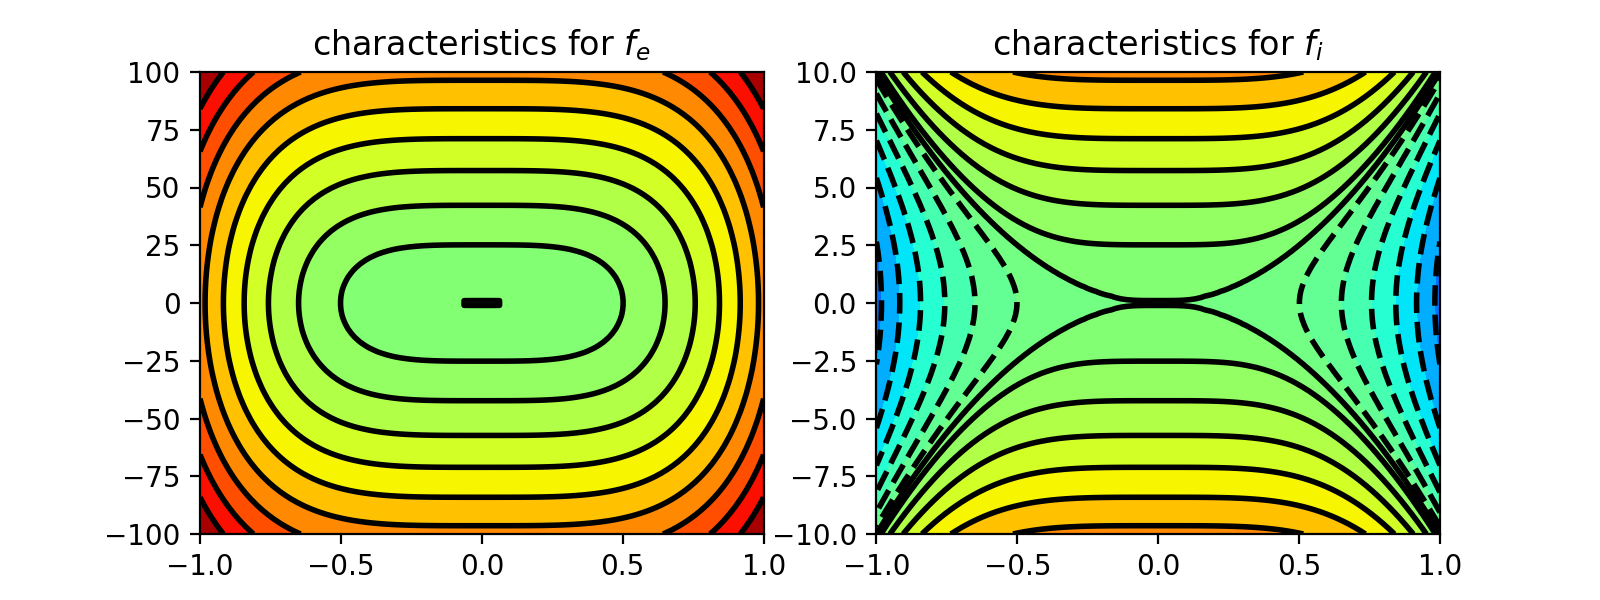
\includegraphics[width=0.9\linewidth]{images/characteristics}
%	\caption{Typical structure of the characteristic lines in the plan $(x,v)$.}
%	\label{fig:characteristics}
%\end{figure}
%
%Let us describe the fixed-point steps. Suppose that a candidate $\varphi^k$ is given. Then:
%\begin{enumerate}
%\item We may deduce the characteristic lines for the equations \cref{eq:sta_model_fi,eq:sta_model_fe}, and compute approximations $f_{i,e}^k$.
%\item By integration on $v$, we may compute $n^k \coloneqq n_i^k - n_e^k$.
%\item The next iterate $\varphi^{k+1}$ is defined as the solution of the Poisson problem \cref{eq:sta_model_phi} with source term $n^k$.
%\end{enumerate}

\section{Numerical results}

The semi-Lagrangian code is written in \texttt{C}; it uses subroutines (translated from \texttt{Fortran}) of the \texttt{selalib} library\footnote{\url{https://selalib.github.io/selalib.html}}. The code works in parallel using \texttt{MPI}.
The finite difference scheme has been written in \texttt{Julia}.

\subsection{1-species validation test case}

We rely on the work of \cite{malkovNonstationaryAntonovSelfgravitating2020} to provide an analytical solution in a 1-species case. Consider the simplified 
%{\textcolor{red}{(NC: pourquoi 'stationary' ?)}} 
model describing the density of particles $f = f(t,x,v)$, and the potential $\varphi=\varphi(t,x)$:
\mysubeq{eq:one_species_model}{
	\partial_t f + v \partial_x f  - \partial_x \varphi \partial_v f &= 0, && (t,x,v) \in \R^+_* \times ]-1,1[ \times \mathbb{R}, \label{sta_1sp_f} \\
	\partial^2_{xx} \varphi &= \int_{v\in\mathbb{R}} f dv, && (t,x) \in \R^+ \times ]-1,1[. \label{sta_phi}
}
The initial and boundary conditions are given by 
\mysubeq{eq:one_species_model_bc}{
	f(0,x,v) \coloneqq f^0(x,v), \quad f(t,x=\pm1, \pm v < 0) &= 0,  \\
	\varphi(t,0) = \partial_x \varphi (t,0) &= 0.  
}
This model may be seen as a particular case of the two-species Vlasov-Poisson \cref{eq:unsta_model}, upon taking the following parameters:
\begin{align*}
	f_i^0 \equiv 0, \quad \nu = 0, \quad \mu = -1, \quad \lambda = 1, \quad f_e^0 = f^0.
\end{align*}
One may verify that \cref{eq:one_species_model} is solved in $\R^+ \times [-1,1] \times \mathbb{R}$ by the following stationary couple:
\begin{align}\label{eq:Malkov_solution}
	f(t,x,v) \coloneqq 
	\begin{cases}
		\frac{1}{\pi} \left(1 - x^2 - v^2\right)^{-1/2} & \text{if } x^2 + v^2 < 1,  \\
		0 & \text{otherwise}, 
	\end{cases} \quad \text{and} \quad
	\varphi(t,x) \coloneqq \frac{x^2}{2}.
\end{align}
It is numerically relevant to extend the Malkov solution \cref{eq:Malkov_solution} to spatial domains $x \in [-1-\varepsilon, 1+\varepsilon]$ by 
\begin{align}\label{eq:Malkov_solution_ext}
	f(t,x,v) \coloneqq 
	\begin{cases}
		\frac{1}{\pi} \left(1 - x^2 - v^2\right)^{-1/2} & \text{if } x^2 + v^2 < 1 \\
		0 & \text{otherwise}
	\end{cases}, \quad \text{and} \quad
	\varphi(t,x) \coloneqq \left\{\begin{array}{c}
	x^2/2,\ \ x<1\\
	|x|-\frac{1}{2},\ x\ge 1
	\end{array}\right.%\min\left(\frac{x^2}{2}, \frac{|x|}{2}\right).
\end{align}

\Cref{fig:malkov_solutions} illustrates the stationary solutions.

\begin{figure}
	\centering
	\renewcommand{\imh}{0.33\linewidth}
	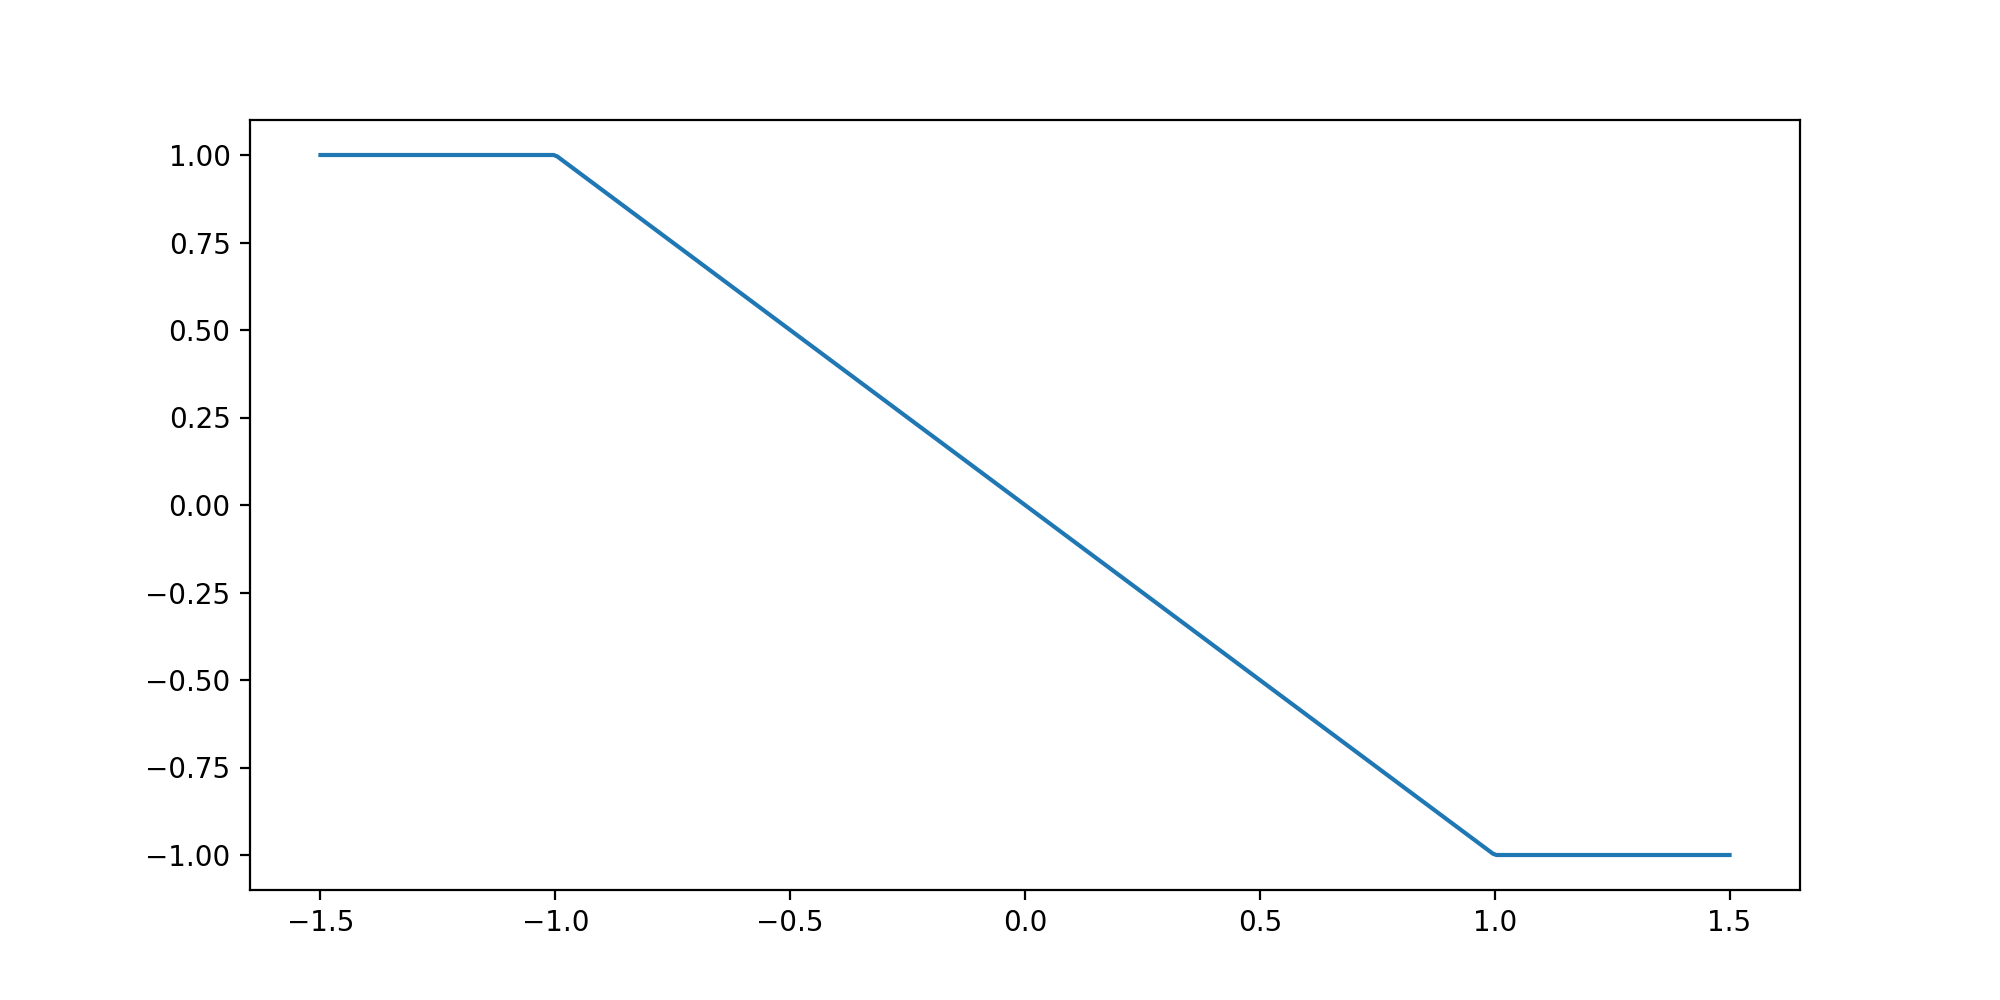
\includegraphics[trim = 50 10 55 30, clip, height=\imh]{images/malkov_solution_Ee}
	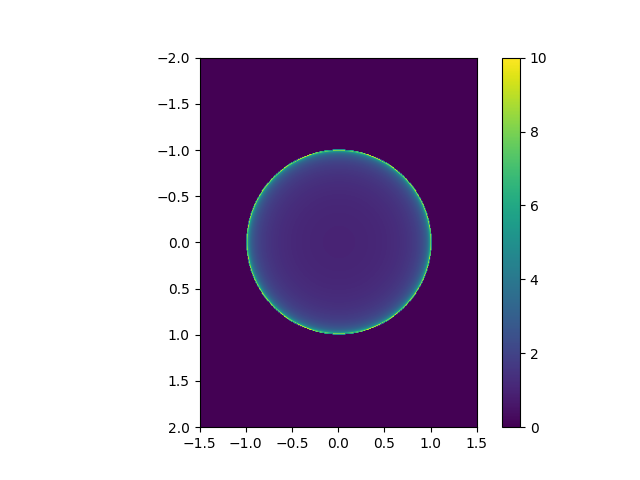
\includegraphics[trim = 100 10 60 30, clip, height=\imh]{images/malkov_solution_fe}
	\caption{Malkov solutions \cref{eq:Malkov_solution_ext} on $[-1.5,1.5]$. Right: electric field $E$. Left: density $f$.}
	\mysubcaption{The electric field is extended outside of $[-1,1]$ by a constant. The density $f$ is represented in the domain $[-1.5,1.5]\times[-2,2]$, and truncated to 10.}
	\label{fig:malkov_solutions}
\end{figure}

\todo{For now, I don't reach order 1. Maybe bug?}

%\begin{figure}[H]
	\begin{table}[H]
	\centering
	\begin{tabular}{|ccc|cc|} \hline
	\multicolumn{3}{|c|}{Parameters} & \multicolumn{2}{c|}{Errors} \\ 
	\cline{1-5} $N_x$ & $N_v$ & $N_t$ & $L^{\infty}$ & $L^1$ \\ 
	\hline \hline 
	100 & 2049 & 1281 & 8.59e-03 & 6.22e-03 \\ \hline 
	200 & 2049 & 1281 & 1.22e-02 & 1.78e-02 \\ \hline 
	400 & 2049 & 1281 & 6.22e-03 & 9.07e-03 \\ \hline 
	800 & 2049 & 1281 & 7.13e-03 & 7.23e-03 \\ \hline \hline
	100 & 4097 & 2561 & 5.65e-03 & 4.92e-03 \\ \hline 
	200 & 4097 & 2561 & 3.88e-03 & 4.70e-03 \\ \hline 
	400 & 4097 & 2561 & 4.08e-03 & 5.77e-03 \\ \hline 
	800 & 4097 & 2561 & 2.39e-03 & 2.93e-03 \\ \hline 
	\end{tabular}
	\caption{DF errors for Malkov test case.}
	\label{tab:Malkov_DF}
\end{table}

	\begin{table}[H]
	\centering
	\begin{tabular}{|ccc|cc|} \hline
	\multicolumn{3}{|c|}{Parameters} & \multicolumn{2}{c|}{Errors} \\ 
	\cline{1-5} $N_x$ & $N_v$ & $N_t$ & $L^{\infty}$ & $L^1$ \\ 
	\hline \hline 
	100 & 201 & 1000 & 1.30e-02 & 1.59e-03 \\ \hline 
	200 & 401 & 1000 & 1.66e-02 & 1.88e-03 \\ \hline 
	400 & 801 & 1000 & 1.88e-02 & 1.35e-03 \\ \hline 
	800 & 1601 & 1000 & 6.15e-03 & 2.66e-04 \\ \hline \hline
	100 & 101 & 100 & 3.19e-02 & 3.45e-03 \\ \hline 
	200 & 201 & 200 & 2.77e-02 & 3.13e-03 \\ \hline 
	400 & 401 & 400 & 6.49e-03 & 4.35e-04 \\ \hline 
	800 & 801 & 800 & 1.51e-02 & 8.50e-04 \\ \hline 
	1600 & 1601 & 1600 & 6.57e-03 & 2.50e-04 \\ \hline \hline
	100 & 2049 & 10000 & 4.06e-03 & 4.62e-04 \\ \hline 
	200 & 2049 & 10000 & 1.72e-02 & 1.40e-03 \\ \hline 
	400 & 2049 & 10000 & 7.88e-03 & 3.90e-04 \\ \hline 
	800 & 2049 & 10000 & 1.12e-02 & 5.37e-04 \\ \hline \hline
	1000 & 201 & 5000 & 1.00e-02 & 3.32e-04 \\ \hline 
	1000 & 401 & 5000 & 1.16e-02 & 5.48e-04 \\ \hline 
	1000 & 801 & 5000 & 5.01e-03 & 1.72e-04 \\ \hline 
	1000 & 1601 & 5000 & 6.34e-03 & 3.25e-04 \\ \hline 
	\end{tabular}
	\caption{SL errors for Malkov test case.}
	\label{tab:Malkov_SL}
\end{table}

%\end{figure}

\subsection{Two species case} % and comparison between (SL) and (FD)}
In this part, we focus on the two-species model \eqref{eq:unsta_model} 
and in the sequel, we use the following physical parameters:
\begin{align}\label{eq:param_simu}
	\lambda = \frac{1}{2}, \quad \mu = \frac{1}{100}, \quad\text{and}\quad \nu = 20.
\end{align}
The initial conditions are chosen as the thermodynamic equilibrium in an infinite spatial domain, or in a domain with periodic condition. The densities are then given by
\begin{align*}
	f_{i}^0 (x,v) \coloneqq \frac{\exp\left(- \frac{v^2}{2}\right)}{\sqrt{2\pi}}, \quad \text{and} \quad f_{e}^0 (x,v) \coloneqq \sqrt{\mu}\frac{\exp\left(- \mu \frac{v^2}{2}\right)}{\sqrt{2\pi}}.
\end{align*}
In order to satisfy the boundary conditions, we multiply $f_{i,e}$ by a mask, defined as
\begin{align*}
	\text{mask}(x,v) \coloneqq \frac{1}{2} \left(\tanh\left(\frac{x - (-0.8)}{0.1}\right) - \tanh\left(\frac{x - 0.8}{0.1}\right)\right).
\end{align*}

\Cref{fig:init_cond} illustrates the resulting initial conditions.
\begin{figure}
	\centering
	\renewcommand{\imh}{0.33\linewidth}
	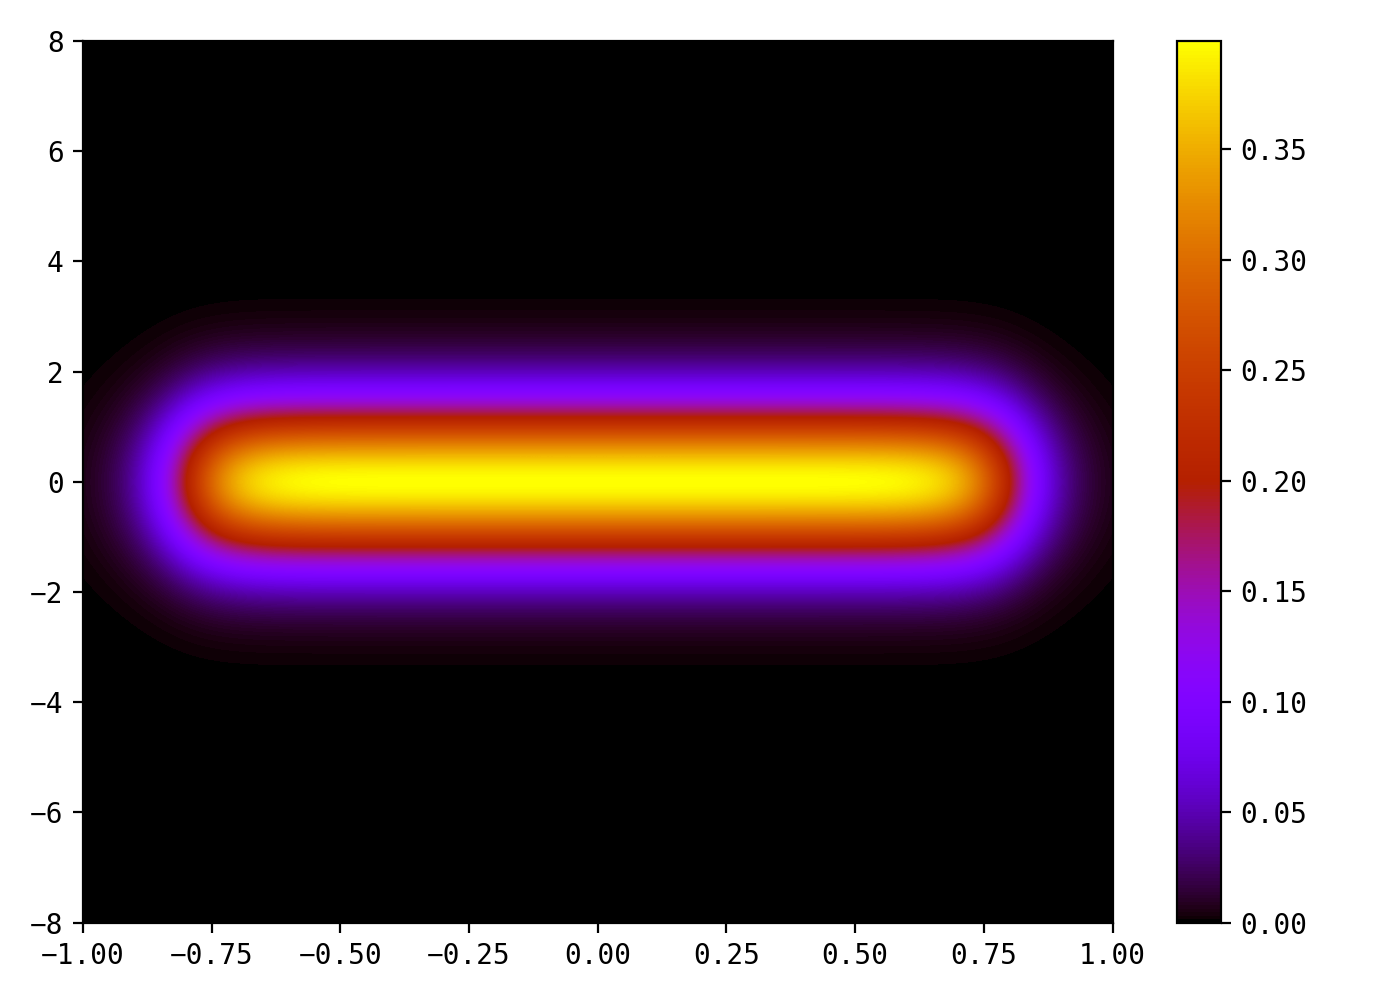
\includegraphics[height=\imh]{images/fi_init}
	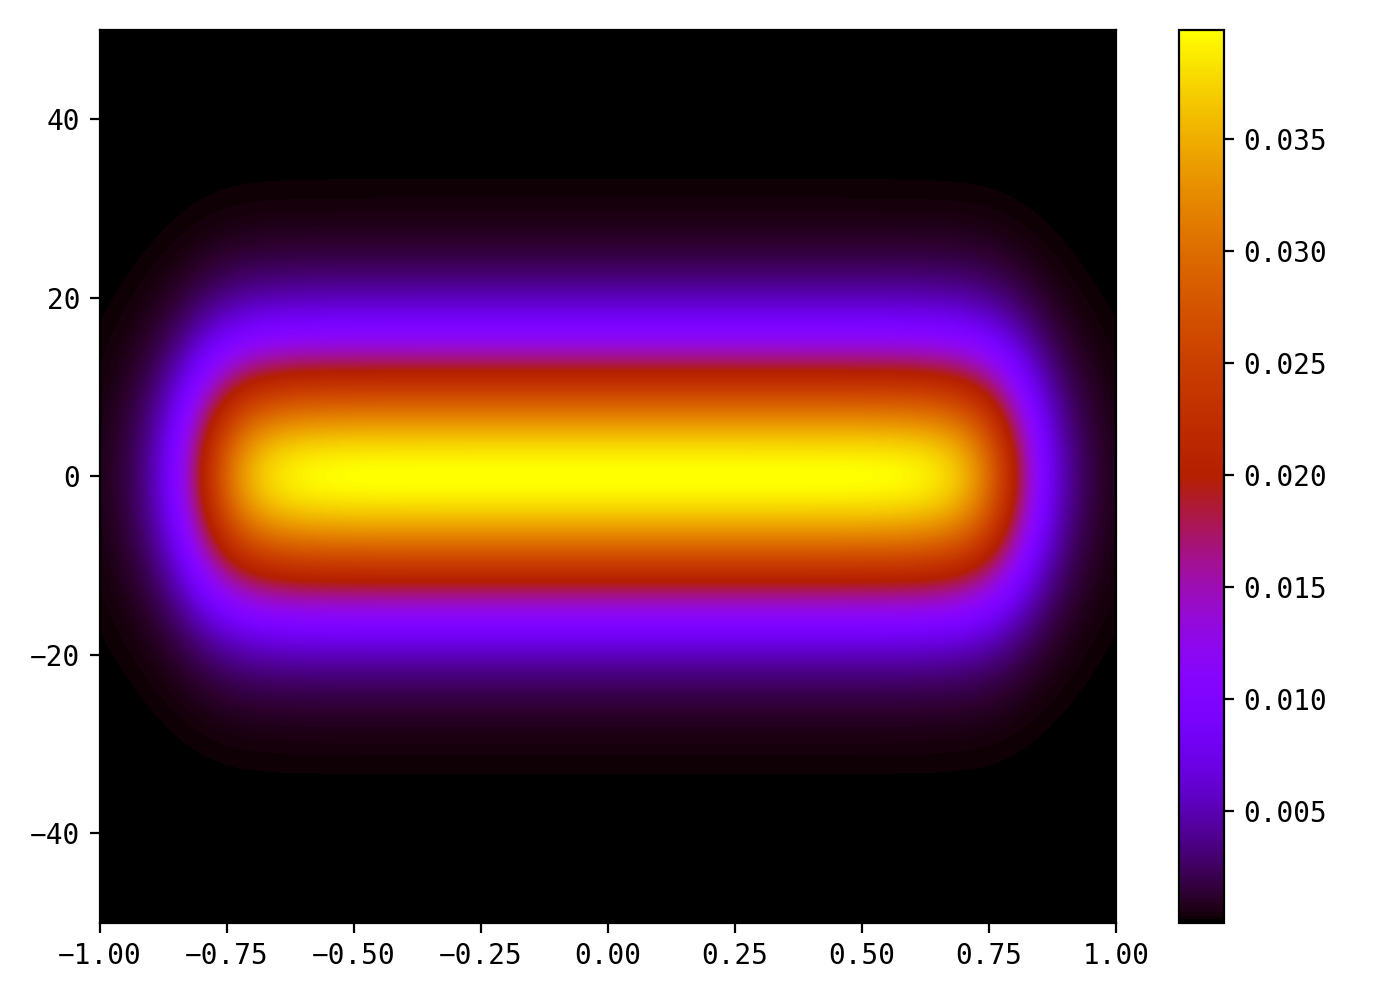
\includegraphics[height=\imh]{images/fe_init}
	\caption{Initial conditions $f_i^0$ (left) and $f_e^0$ (right).}
	\label{fig:init_cond}
\end{figure}


The simulations run over the spatial domain $x \in [-1,1]$. The semi-Lagrangian (SL) code computes the electron velocities on $v_e \in [-60, 60]$, and ion velocities on $v_i \in [-50, 50]$. The finite differences (FD) code uses the same mesh for ions and electrons, chosen as $v\in[-60,60]$. To simplify the comparison, visualisations of $f_i$ are restricted to the coordinates $f_{i,j,k}$ such that $v_k \in [-5,5]$.
For the finite differences code, we use $N_x=512$, $N_{v_e}=N_{v_i}=513$; the time step is computed in order to satisfy the CFL condition; a further time step is used for terminating to the final time $T$.  
For the semi-Lagrangian code, we will use

\begin{table}[H]
	\centering
	\begin{tabular}{|c|c|c|c|c|} \hline
	Run & $N_x$ & $N_{v_i}$ & $N_{v_e}$ & $\Delta t$ \\ 
	\hline \hline 
	Run0 & 512 & 513 & 513 & 0.000250 \\ \hline 
	Run1 & 256 & 2049 & 8193 & 0.000250 \\ \hline 
	Run2 & 1024 & 2049 & 8193 & 0.000250 \\ \hline 
	Run3 & 1024 & 2049 & 8793 & 0.000025 \\ \hline 
	\end{tabular}
	\label{tab:runs}
\end{table}


%\begin{itemize}
%\item Run0: $N_x=512$, $N_{v_e}=N_{v_i}=513$, $\Delta t = 0.00025$,
%\item Run1: $N_x=256$, $N_{v_e}=8193$ and $N_{v_i}=2049$, $\Delta t = 0.00025$,
%\item Run2: $N_x=1024$, $N_{v_e}=8193$ and $N_{v_i}=2049$, $\Delta t = 0.00025$,
%\item Run3: $N_x=1024$, $N_{v_e}=8193$ and $N_{v_i}=2049$, $\Delta t = 0.000025$.
%\end{itemize}

For the SL scheme, we always use $d=8$ with periodic boundary conditions for the interpolation in velocity, and $k_b=1$ together with $d=2$ for the spatial interpolation.
Lagrange interpolation of degree $3$  (that is, $d=1$) is used for passing from the ion velocity mesh to the electron velocity mesh (which is needed for the ionization step).

As diagnostics, we represent the electric field $E$, the charge density $n=n_i-n_e$, the ion distribution function $f_i$ and the electron distribution function $f_e$ at different times $T\in \left\{0.1,0.2,1,2,5,20\right\}$.

\paragraph{Short time}

We first look at the results for short times: $T=0.1$ (Figure \ref{fig:compT01}) and $T=0.2$ (Figure \ref{fig:compT02}). For the semi-Lagrangian code, we use the parameters of Run2, which gives a reference solution.
We see that the results are very similar with the FD code for $T=0.1$, which permits to validate the results by cross comparisons. For $T=0.2$, differences begin to appear; the sharp profile of $f_e$ is not well
reproduced by the FD scheme which has also a coarser mesh. We can see also the differences on the charge density.

%The same simulation at time $T=0.1$ shows a greater divergence between both methods. The electric field does not have the same extremal values, and the comparison of $\rho$ reveals a difference of variations. The approximations of the ion density $f_i$ seem quite similar, but the shape of the electric density $f_e$ differs: the semi-lagrangian code produces sharper approximation and a more elongated profile.

\paragraph{Long time}

Now, we turn to the long-term simulations, with $T=20$, on Figure \ref{fig:compT20}.  %Here, we free the semi-Lagrangian code from the artificial CFL condition imposed for fair comparisons. \Cref{fig:compT200} illustrates the behavior of both codes on long time, with parameters given by \cref{eq:param_simu}. 
%
The finite difference code suffers from numerical diffusion, and the approximations of $f_i$ and $f_e$ are very damped. Electric field and charge density are really different.
On the contrary, the SL scheme gives much better results (in comparison with refined runs, as we will see later), while it uses the same number of points. We can distinguish a little degradation of the symmetry, by looking at the charge density.
%almost everywhere reduced to 0. %The point $(x=0,v=0)$ stands out, since it is an equilibrium point: the value $f_e(t,0,0)$ is constant with respect to $t$ (both in the continuous model, and in the discrete model provided $(x=0,v=0)$ belongs to the mesh), and 
%\begin{align*}
%	\partial_t f_i (t,0,0) = f_e(t,0,0),  \quad \text{so that} \quad f_i(t,0,0) = f_i(0,0,0) + t f_e(0,0,0).
%\end{align*}
%This explains the results of \cref{fig:compT200}. The value $f^n_{e,j_0,k_0} \simeq f_e(T,0,0)$ is stationary, but the maximum of $f_e^n$ outside a small neighbourhood of $(x=0,v=0)$ is 0 at machine precision.
%%The numerical maximum of $f_i$ is equal to $159.97581842617524$, and the error with respect to $f_i(0,0,0) + (T=200) \times (\nu = 20) \times f_e(0,0,0)$ is of order $10^{-8}$. 
%The value $f^n_{i,j_0,k_0} \simeq f_i(T,0,0)$ is not taken into account in the colormap, since
%\begin{align*}
%	\max_{j,k} f^n_{i,j,k} = f^n_{i,j_0,k_0} = 159.97581842617524, \quad \text{and} \quad \left|f^n_{i,j_0,k_0} - (f^0_{i,j_0,k_0} + T \nu f^0_{e,j_0,k_0})\right| = 8.98 \times 10^{-9}.
%\end{align*}
%
%At the opposite, the semi-Lagrangian scheme does not produce vanishing approximations. 


\paragraph{Looking for a reference solution} %Numerical results for the SL code for different discretizations}

It is not easy to find a reference solution, as we look for long time solution, and the Vlasov equation is prone to filamentation. We have here also the problem electrons and ions have different time scales, which implies that short time steps have to be used in order to be able to follow the dynamics (even if we use here a semi-Lagrangian scheme, whose time step is not restricted by the strong CFL condition
of the finite difference scheme).

It is interesting to notice that we can have converged solutions for a fixed time step, taking for exemple $\Delta t = 0.0025$ (or even $\Delta t =0.025$), but the corresponding solution is then not (at all) converged in time
(results are shown on Figure \ref{fig:comp_temps2}; we can remark that the results on charge density can be quite different; looking at the electron distribution function, we see some shifting
of the solution, and even more changes for $\Delta t =0.025$). So we have diminished the time step to $\Delta t = 0.00025$, and the comparison with the same simulations with  $\Delta t = 0.000025$ on Figure \ref{fig:comp_temps} 
is now much similar, which indicates that the 
time step is now fine enough. Note that for semi-Lagrangian schemes, taking the smallest possible time step does not necessarily lead to a better result (due to accumulation of errors, as the number of interpolations 
increases).

We choose to use a very fine discretization in velocity for the electron by taking $N_v=8193$ (some results, not shown, with $N_v=16385$ have lead to indistinguishable results).
We then make vary $N_x$ and $N_{v_i}$; we remark that $N_x$ can be quite lower and $N_{v_i}$ a little lower also, as we have similar results taking $(N_x,N_{v_i})=(256,2049)$ and 
$(N_x,N_{v_i})=(1024,4097)$, as we can see on Figure \ref{fig:comp_phasespace} (the first one is more diffusive which is coherent). 
%We would like to have a solution that is 

%We want here to compare the semi-Lagrangian code with different discretizations.
%We have here no exact solution at hand to validate the code; so we validate it by comparing the numerical parameters. We restrict here to final time $T=20$ and look for "converged" numerical parameters.
%It is beneficial that the code is parallel (remap strategy of the selalib project\footnote{\url{https://selalib.github.io/selalib.html}}); in practice we do the simulations on a labtop or in the mesocentre of Marseille
%($16$ cores for interactive mode and $32$ cores for submitted jobs, which can be prone to delays, depending on the queue).
%
%We choose to use a high number for the electron density, by taking $N_v=8193$, 
%and we study the change for $N_x$ and $N_{v_i}$, taking first $N_x=256$ and $N_{v_i}=2049$, and then taking $N_x=1024$ and  $N_{v_i}=4097$.
%Numerical results are shown on Figure \ref{fig:comp_phasespace}. We clearly see that the results are quite similar, with a more diffusive solution for the coarser mesh, which is encouraging.
%
%On Figure \ref{fig:comp_temps}, we study the validity of the time discretization, changing the value of $\Delta t$, which goes from
%$\Delta t=0.00125$ to $\Delta t=0.000125$. We again see that results are very similar, which is a good point.
%
%
%The ion density and the electric field seem not to change much; but the electron density is varying a lot and becomes more and more complex with respect to time,
%and filaments appear. Note that we have to take quite small time steps, as we have chosen $\mu=1/100$, which makes the study more difficult, but it is nearer to more physically relevant parameters. 
%We have chosen also a high number for $N_{v_e}$; this permits to better keep the symmetry, without imposing it a priori (which is in fact possible, by a symmetrization of $\rho$).

We remark also that the spatial interpolation does not lead to unstable results, which can occur sometimes when extrapolation is used (see \cite{badsiNumericalStabilityPlasma}).
We have used an odd number of points in order to prevent from having  $0$ as a mesh point, which would lead to increase of the value at constant rate, in the ionization step.

The study of the numerical equilibrium and the study of the behavior of the ion density around $(0,0)$, which is quite complex at equilibrium, are not tackled here and are out of the scope of this work.


%\begin{figure}
%	\centering
%	\newcommand{\rootSL}{../code_SL/}
%%	\newcommand{\rootFD}{../../DynamicElectricSheath.jl/data/two_species/}
%	\newcommand{\rootFD}{../temp_res_DF/}
%	\newcommand{\dirSL}{run_comp_short_time_2sp_Nx1000_Nvi2001_Nve2001_Nt1563}
%	\newcommand{\dirFD}{run_comp_short_time_2sp_Nx1000_Nv2000_Nt1563}
%	\renewcommand{\imh}{0.33\linewidth}
%	
%	\begin{subfigure}{\textwidth}
%		\centering
%		\includegraphics[height=\imh]{\rootFD\dirFD/comp_E_\dirSL.png}
%		\includegraphics[height=\imh]{\rootFD\dirFD/comp_rho_\dirSL.png}
%		\caption{Electric field (left) and density $\rho$ (right)}
%		\label{subfig:compT0025_E_rho}
%	\end{subfigure}
%	
%	\begin{subfigure}{\textwidth}
%		\centering
%		\includegraphics[height=\imh]{\rootFD\dirFD/fi}
%		\includegraphics[height=\imh]{\rootSL\dirSL/python_diags/fi}
%		\caption{Ion density}
%		\label{subfig:compT0025_ion}
%	\end{subfigure}
%	\begin{subfigure}{\textwidth}
%		\centering
%		\includegraphics[height=\imh]{\rootFD\dirFD/fe}
%		\includegraphics[height=\imh]{\rootSL\dirSL/python_diags/fe}
%		\caption{Electron density}
%		\label{subfig:compT0025_electron}
%	\end{subfigure}
%	\caption{Comparison between finite differences (left) and semi-Lagrangian (right) at $T=0.025$.}
%	\label{fig:compT0025}
%\end{figure}  
%
%\Cref{fig:compT0025} illustrates the very short-time behaviour of both codes. At time $t=0$, the initial conditions are chosen so that $E = \rho = 0$, corresponding to a neutral plasma. The initial velocity field is then given by $(v, 0)$, and we observe the shear of the initial conditions. The electric field conserve the same variations through both codes, with a difference in scale.

%\begin{figure}
%	\centering
%	\newcommand{\rootSL}{../code_SL/}
%%	\newcommand{\rootFD}{../../DynamicElectricSheath.jl/data/two_species/}
%	\newcommand{\rootFD}{../temp_res_DF/}
%	\newcommand{\dirSL}{run_comp_short_time_2sp_Nx1000_Nvi2001_Nve2001_Nt6250}
%	\newcommand{\dirFD}{run_comp_short_time_2sp_Nx1000_Nv2000_Nt6250}
%	
%	\renewcommand{\imh}{0.33\linewidth}
%	
%	\begin{subfigure}{\textwidth}
%		\centering
%		\includegraphics[height=\imh]{\rootFD\dirFD/comp_E_\dirSL.png}
%		\includegraphics[height=\imh]{\rootFD\dirFD/comp_rho_\dirSL.png}
%		\caption{Electric field (left) and density $\rho$ (right)}
%		\label{subfig:compT01_E_rho}
%	\end{subfigure}
%	
%	\begin{subfigure}{\textwidth}
%		\centering
%		\includegraphics[height=\imh]{\rootFD\dirFD/fi}
%		\includegraphics[height=\imh]{\rootSL\dirSL/python_diags/fi}
%		\caption{Ion density}
%		\label{subfig:compT01_ion}
%	\end{subfigure}
%	\begin{subfigure}{\textwidth}
%		\centering
%		\includegraphics[height=\imh]{\rootFD\dirFD/fe}
%		\includegraphics[height=\imh]{\rootSL\dirSL/python_diags/fe}
%		\caption{Electron density}
%		\label{subfig:compT01_electron}
%	\end{subfigure}
%	\caption{Comparison between finite differences (left) and semi-Lagrangian (right) at $T=0.1$.}
%	\label{fig:compT01}
%\end{figure}  

\begin{figure}
	\centering
	\newcommand{\rootSL}{../code_SL/}
%	\newcommand{\rootFD}{../../DynamicElectricSheath.jl/data/two_species/}
	\newcommand{\rootFD}{../temp_res_DF/}
	\newcommand{\dirSL}{run_comp_short_time_2sp_Nx1000_Nvi2001_Nve2001_Nt6250}
	\newcommand{\dirFD}{run_comp_short_time_2sp_Nx1000_Nv2000_Nt6250}
	
	\renewcommand{\imh}{0.24\textheight}
	\renewcommand{\imw}{0.45\linewidth}
	\begin{subfigure}{\textwidth}
		\centering
		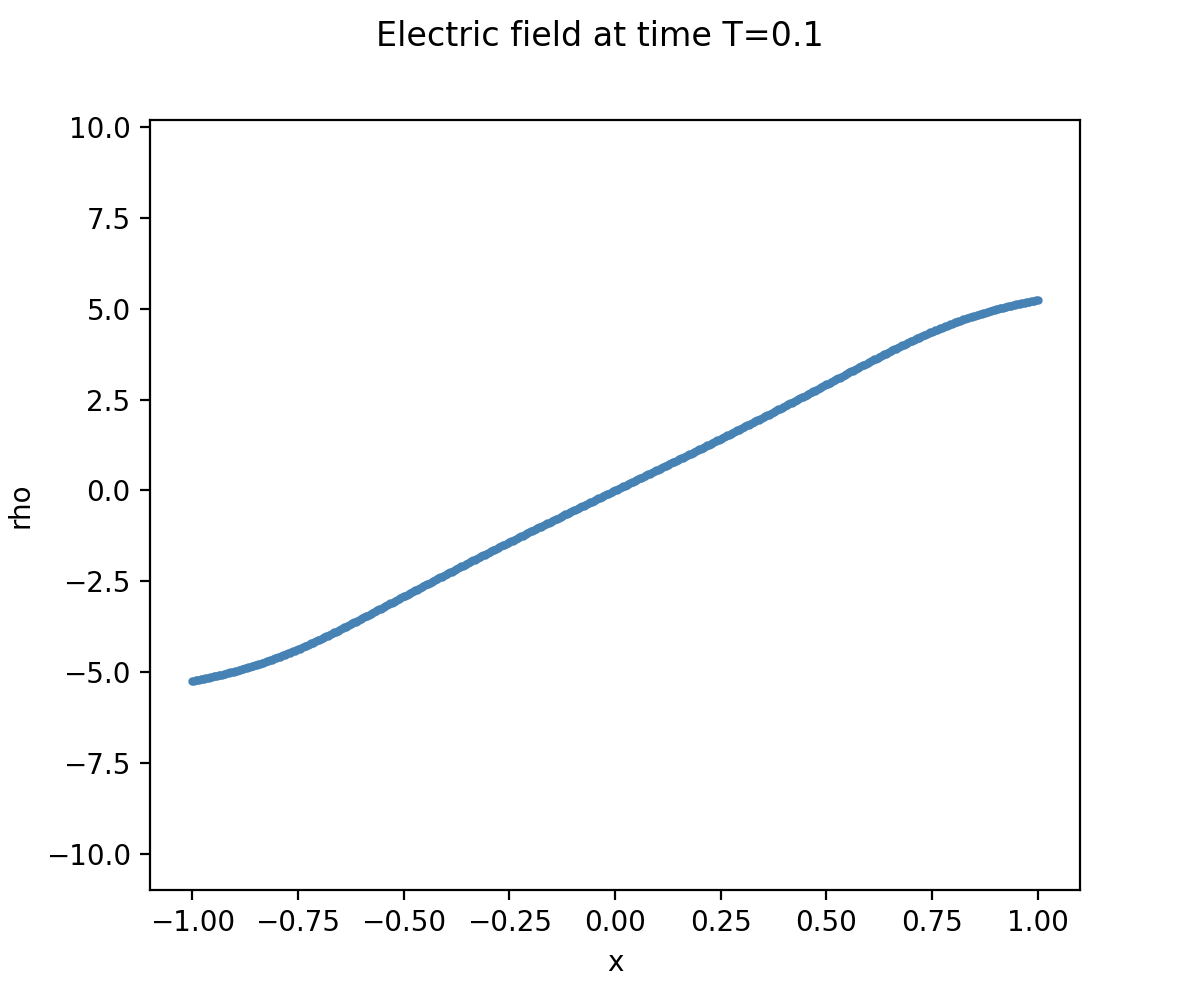
\includegraphics[height=\imh,width=\imw]{images/ET0p1_FD.png}
		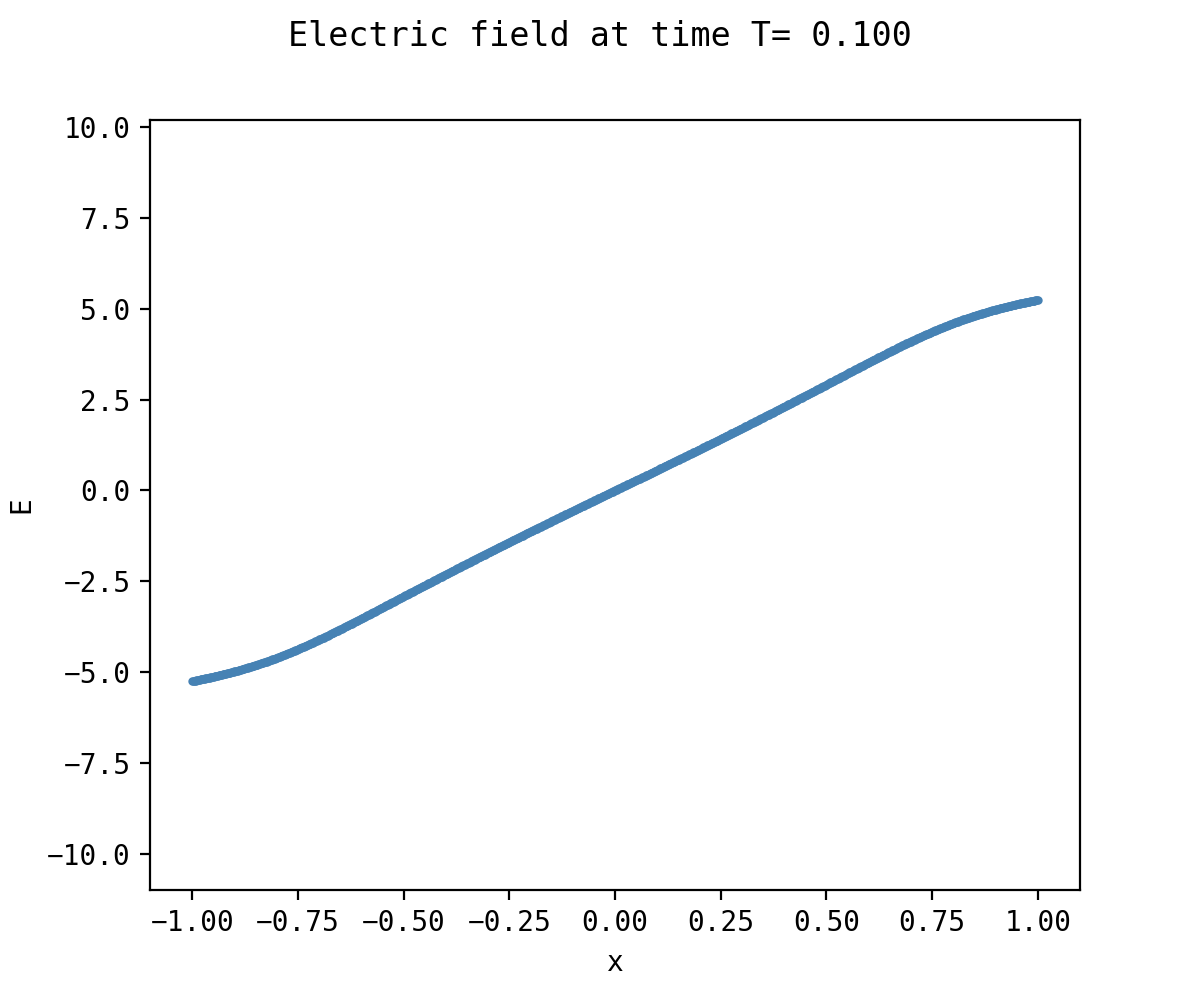
\includegraphics[height=\imh,width=\imw]{images/ET0p1.png}
		\caption{Electric field }
		\label{subfig:compT01_E}
	\end{subfigure}

	\begin{subfigure}{\textwidth}
		\centering
		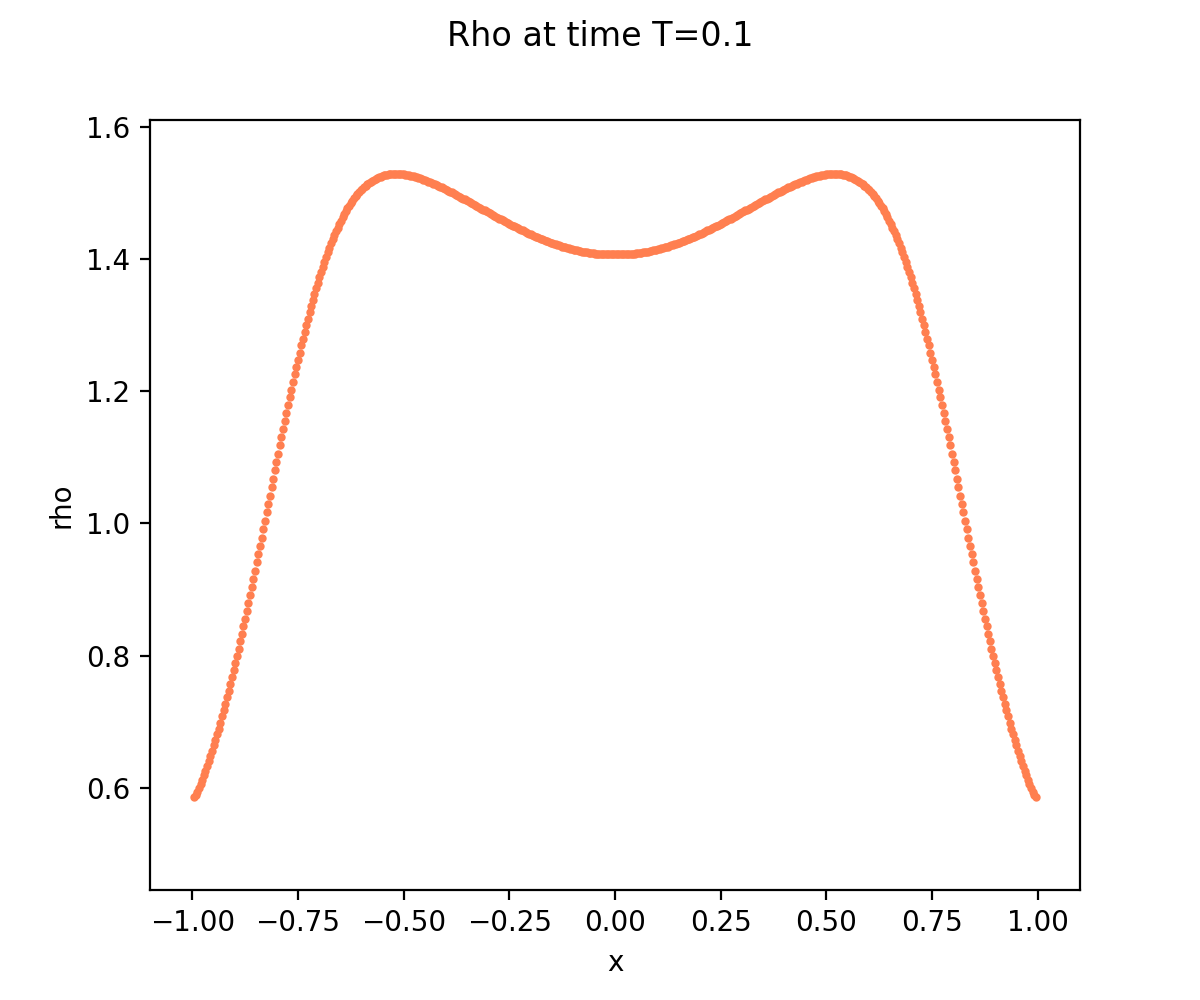
\includegraphics[height=\imh,width=\imw]{images/rhoT0p1_FD.png}
		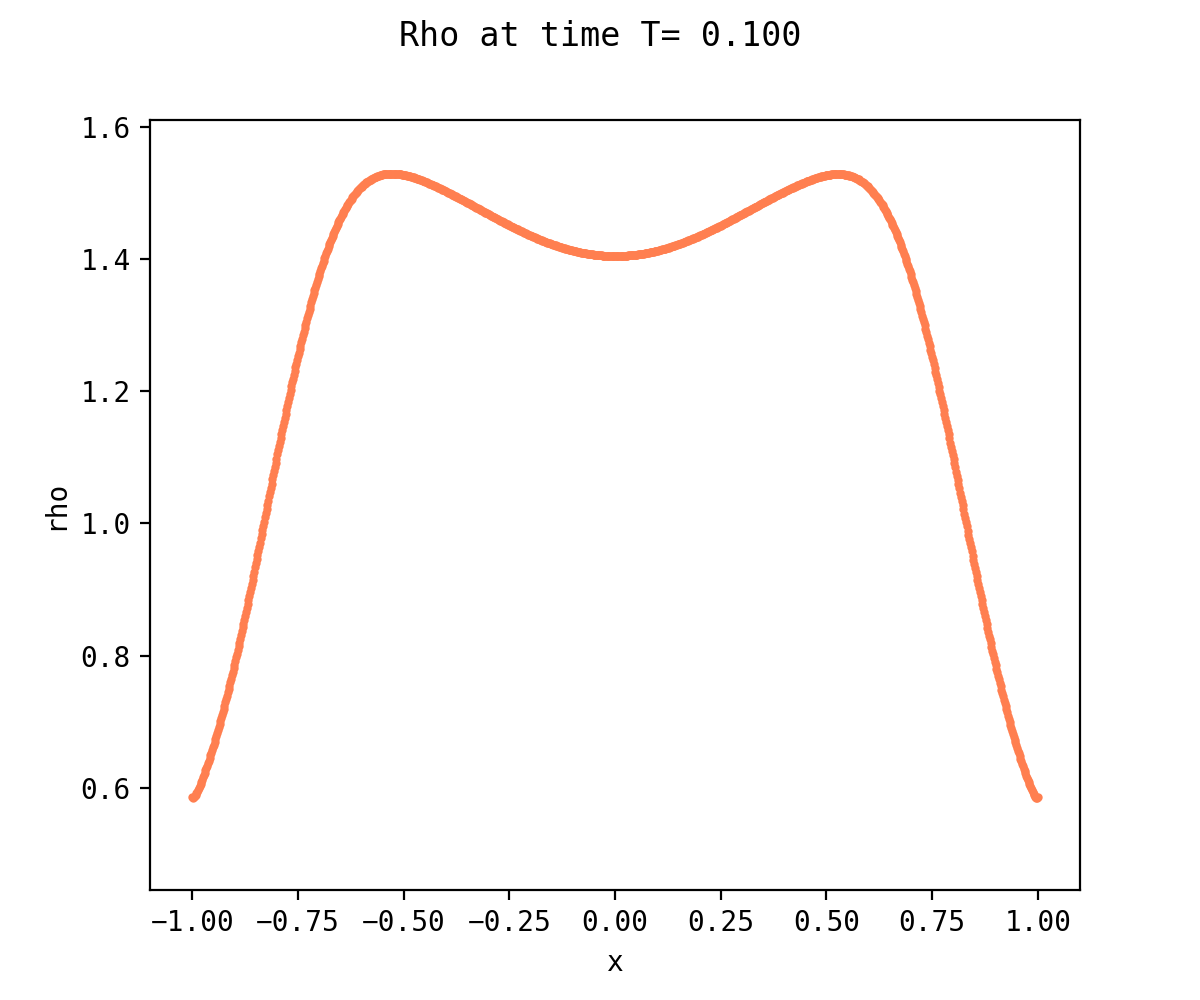
\includegraphics[height=\imh,width=\imw]{images/rhoT0p1.png}
		\caption{Density $\rho$}
		\label{subfig:compT01_rho}
	\end{subfigure}
	
	\begin{subfigure}{\textwidth}
		\centering
		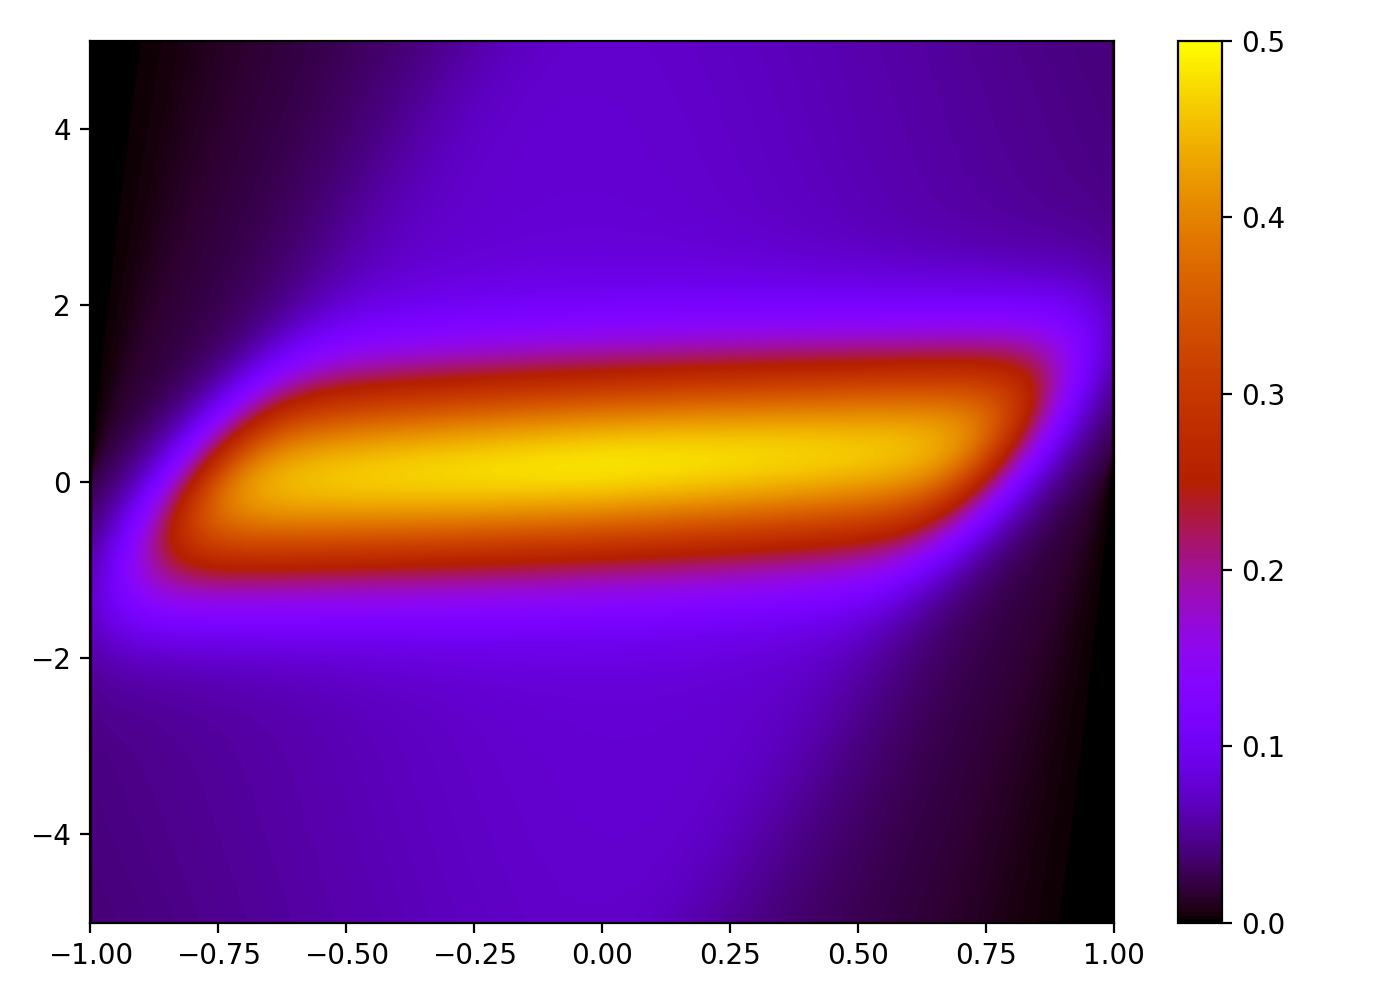
\includegraphics[height=\imh,width=\imw]{images/fiT0p1_FD.png}
		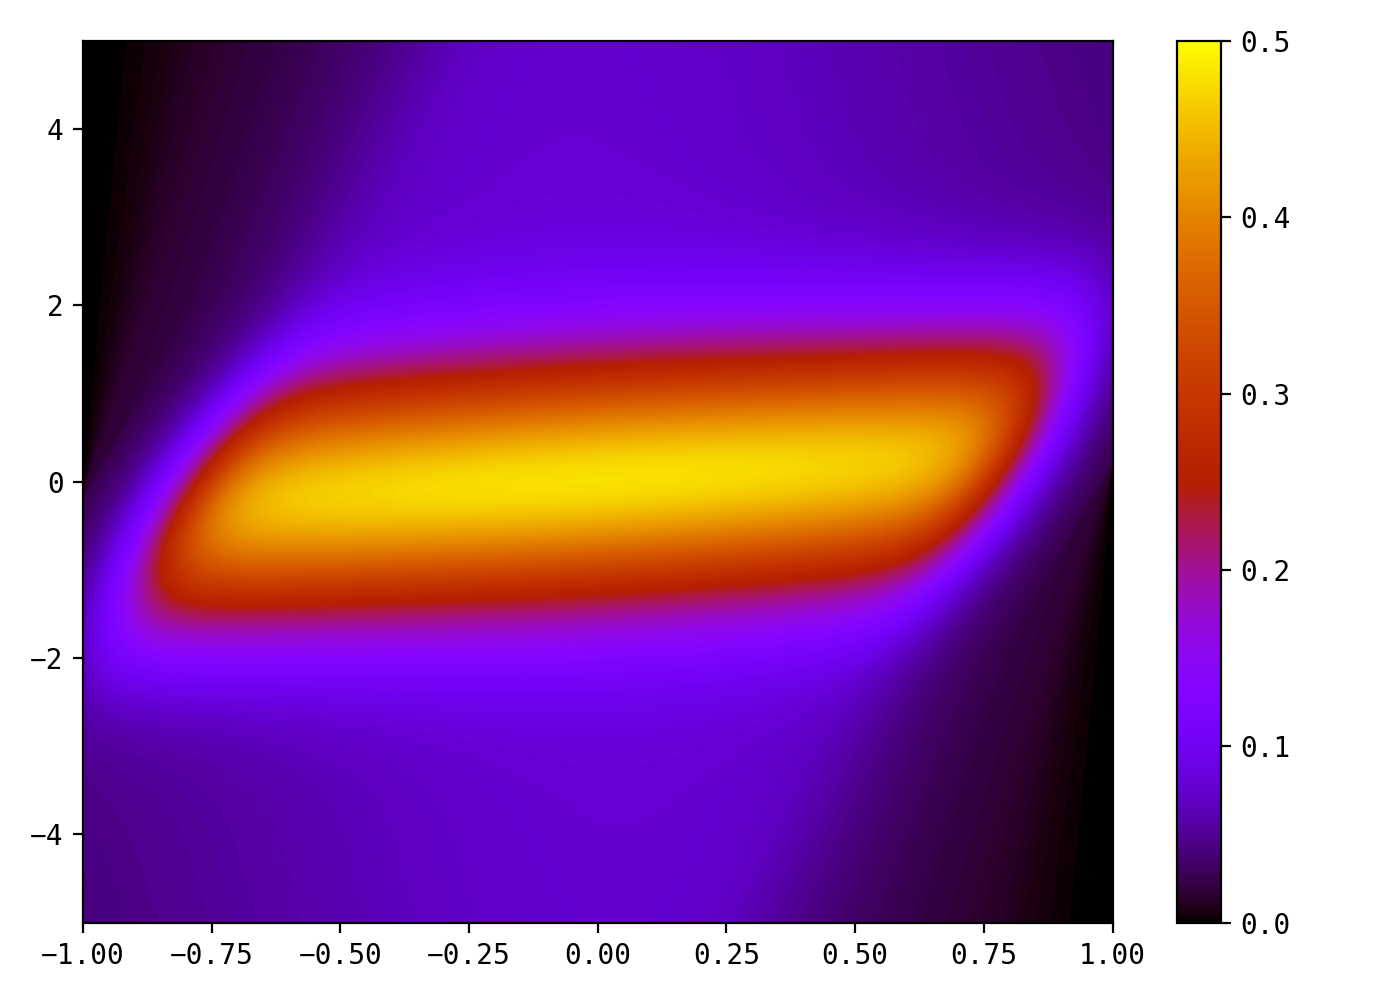
\includegraphics[height=\imh,width=\imw]{images/fiT0p1.png}
		\caption{Ion distribution function}
		\label{subfig:compT01_ion}
	\end{subfigure}
	\begin{subfigure}{\textwidth}
		\centering
		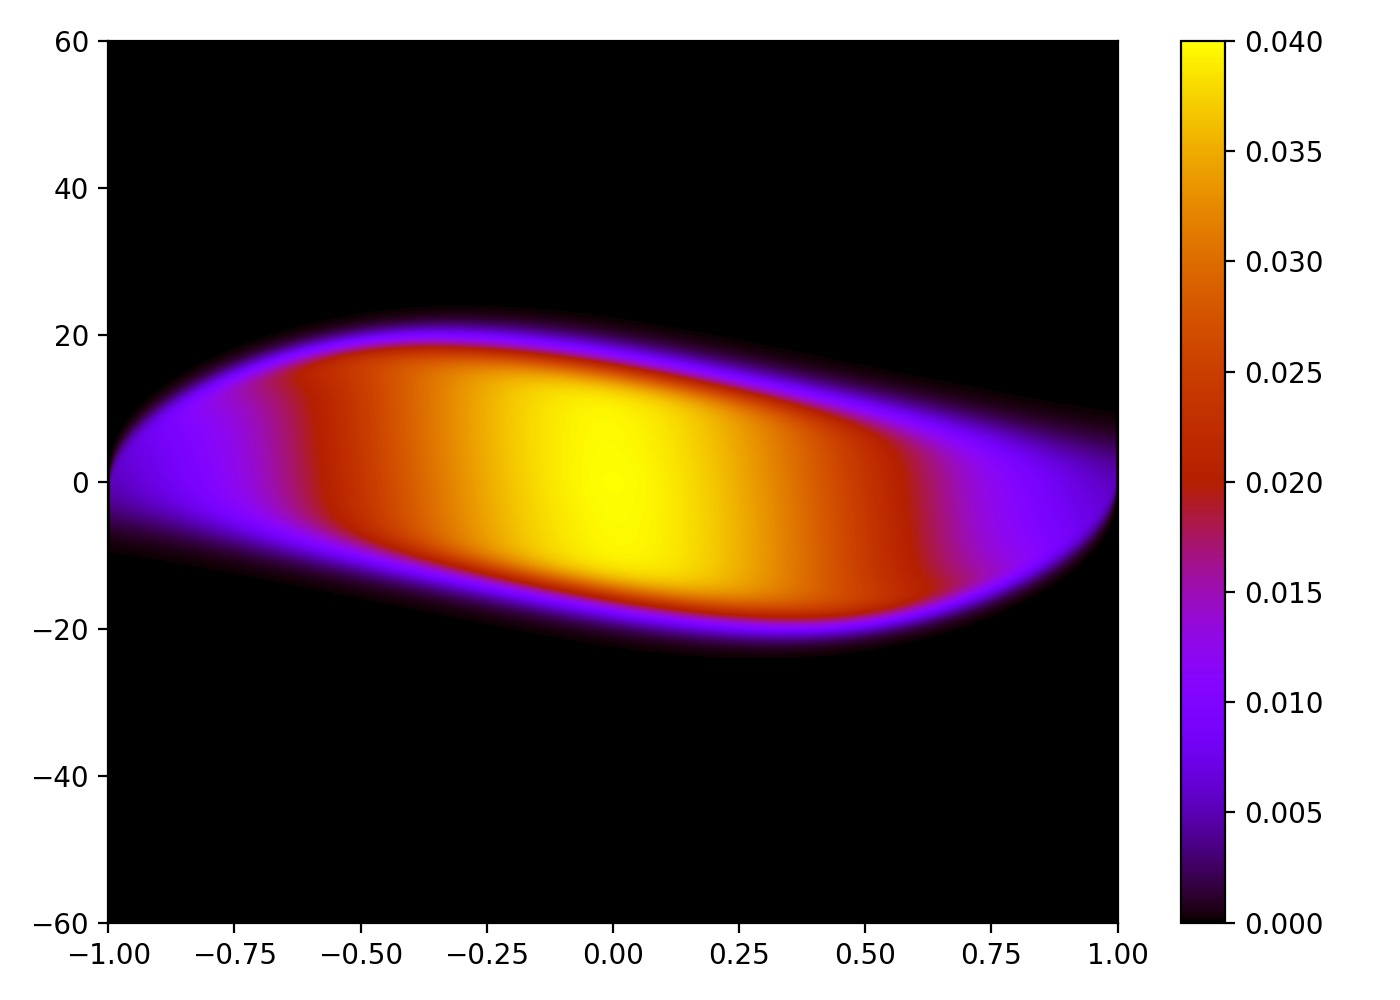
\includegraphics[height=\imh,width=\imw]{images/feT0p1_FD.png}
		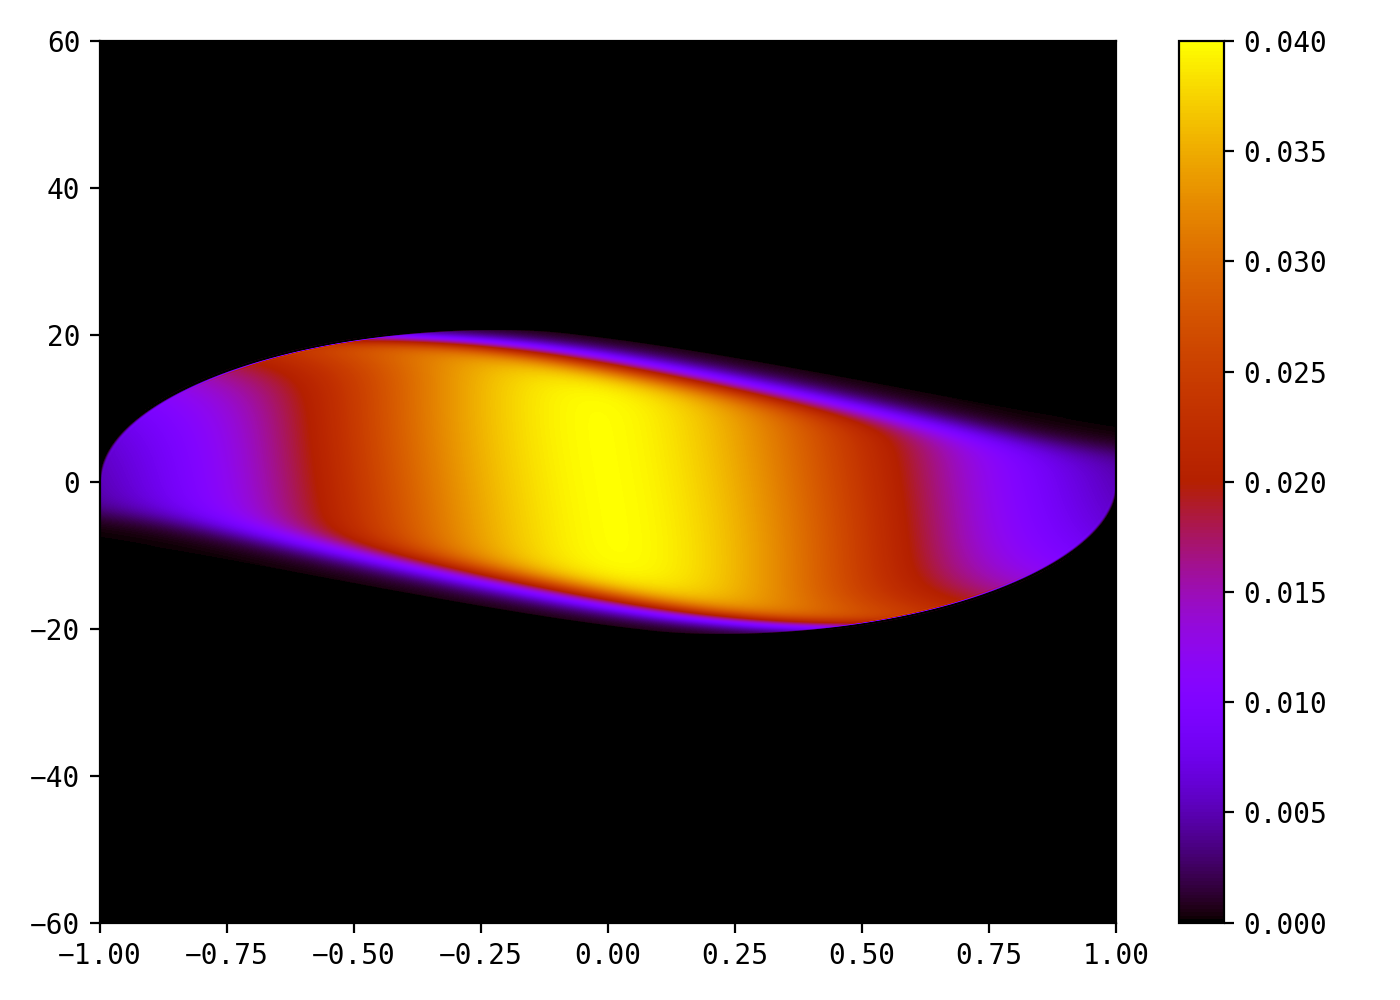
\includegraphics[height=\imh,width=\imw]{images/feT0p1.png}
		\caption{Electron distribution function}
		\label{subfig:compT01_electron}
	\end{subfigure}
	\caption{Comparison between finite differences (left) and semi-Lagrangian (right) at $T=0.1$. The Semi-Lagrangian code uses parameters of Run2.}
	\label{fig:compT01}
\end{figure}  

\begin{figure}
	\centering
	\newcommand{\rootSL}{../code_SL/}
%	\newcommand{\rootFD}{../../DynamicElectricSheath.jl/data/two_species/}
	\newcommand{\rootFD}{../temp_res_DF/}
	\newcommand{\dirSL}{run_comp_short_time_2sp_Nx1000_Nvi2001_Nve2001_Nt6250}
	\newcommand{\dirFD}{run_comp_short_time_2sp_Nx1000_Nv2000_Nt6250}
	
	\renewcommand{\imh}{0.24\textheight}
	\renewcommand{\imw}{0.45\linewidth}
	
	\begin{subfigure}{\textwidth}
		\centering
		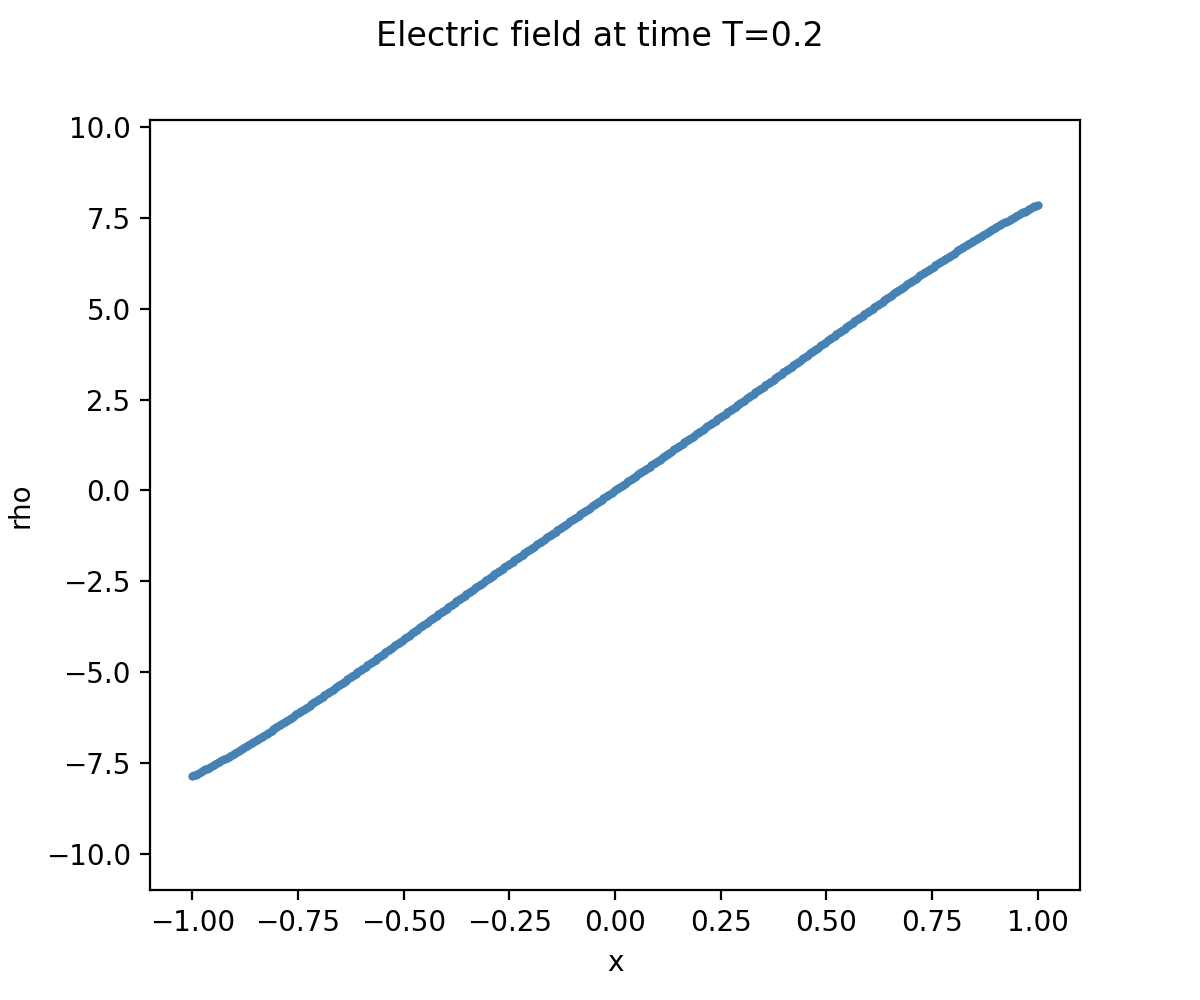
\includegraphics[height=\imh,width=\imw]{images/ET0p2_FD.png}
		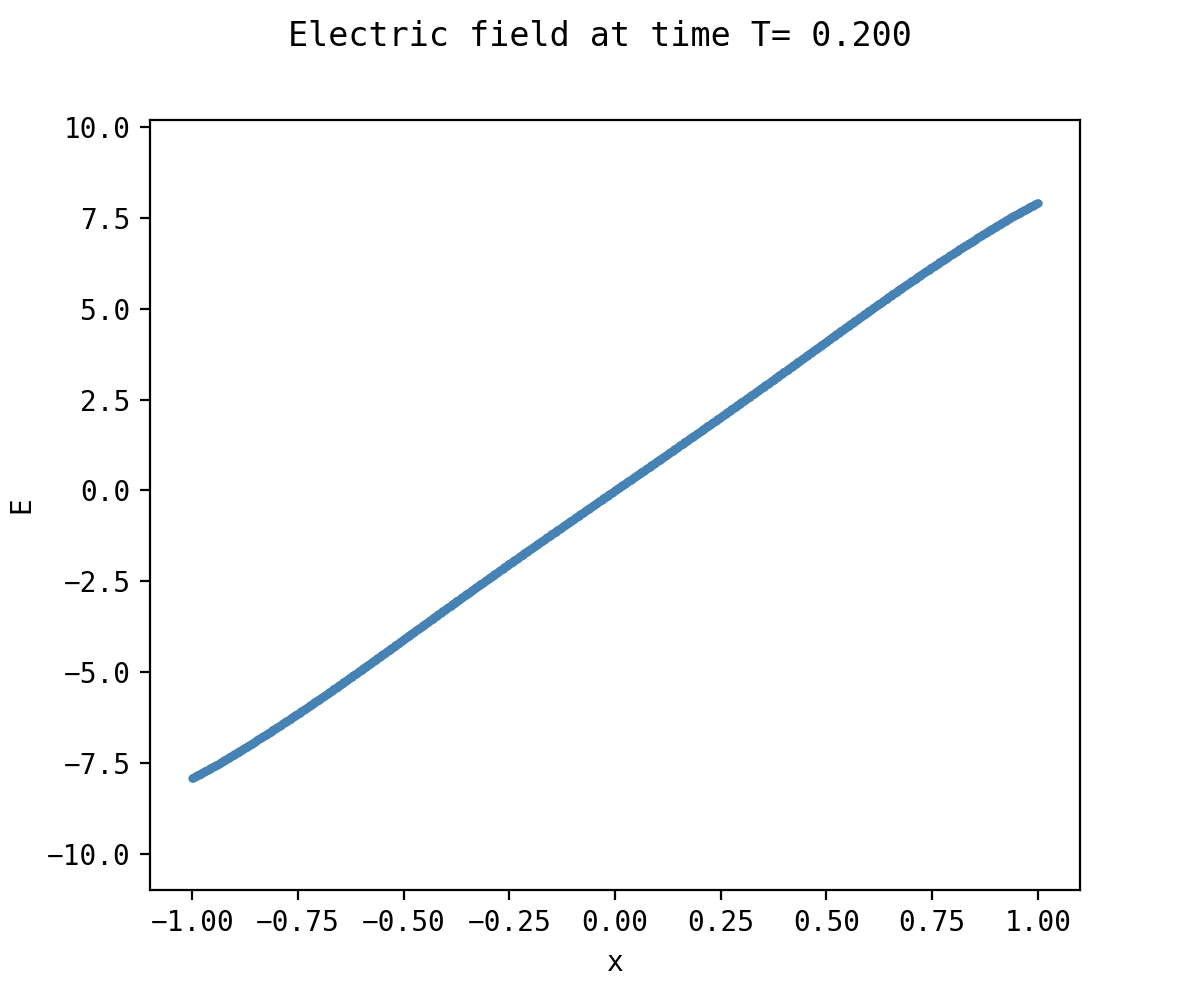
\includegraphics[height=\imh,width=\imw]{images/ET0p2.png}
		\caption{Electric field }
		\label{subfig:compT02_E}
	\end{subfigure}

	\begin{subfigure}{\textwidth}
		\centering
		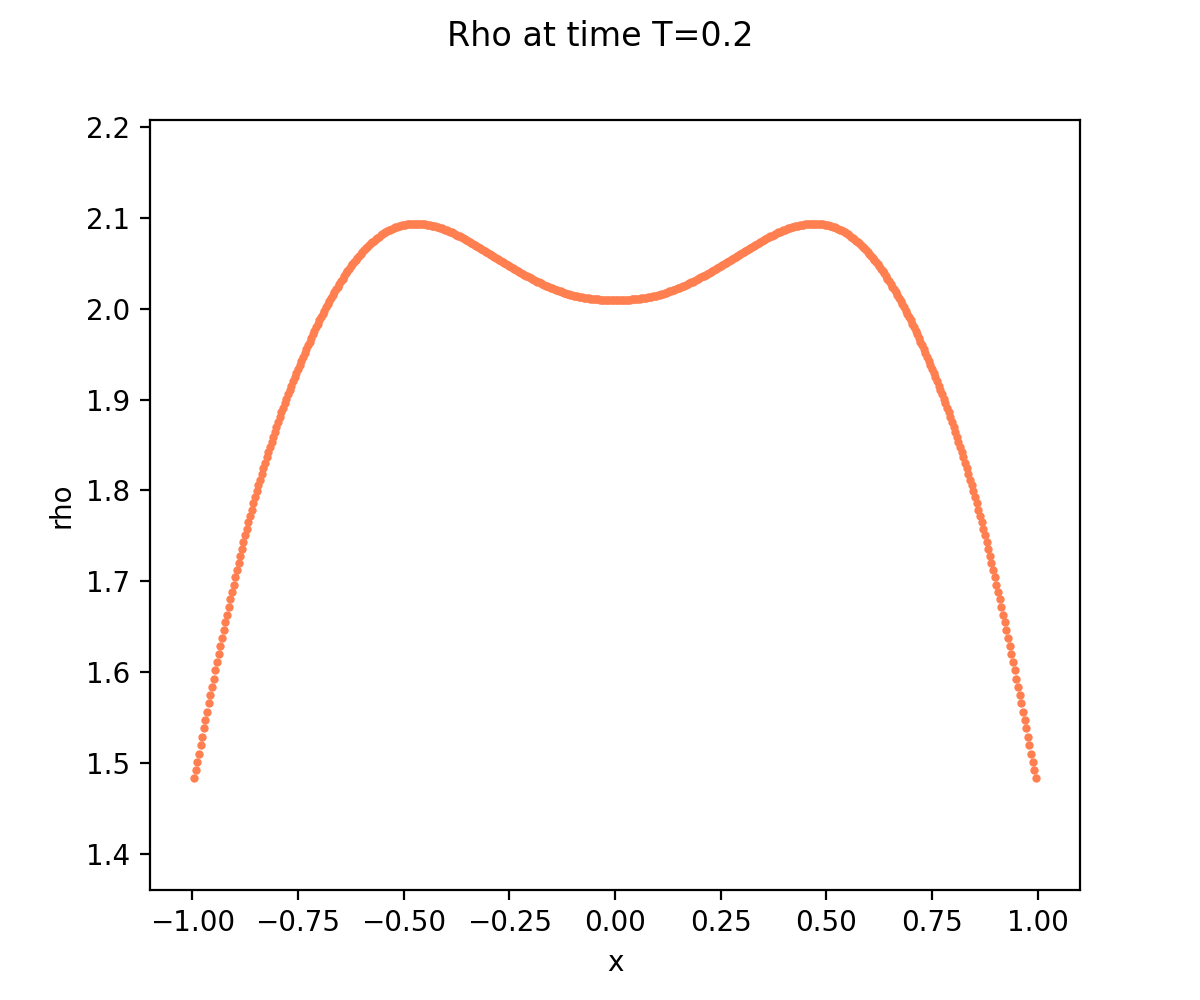
\includegraphics[height=\imh,width=\imw]{images/rhoT0p2_FD.png}
		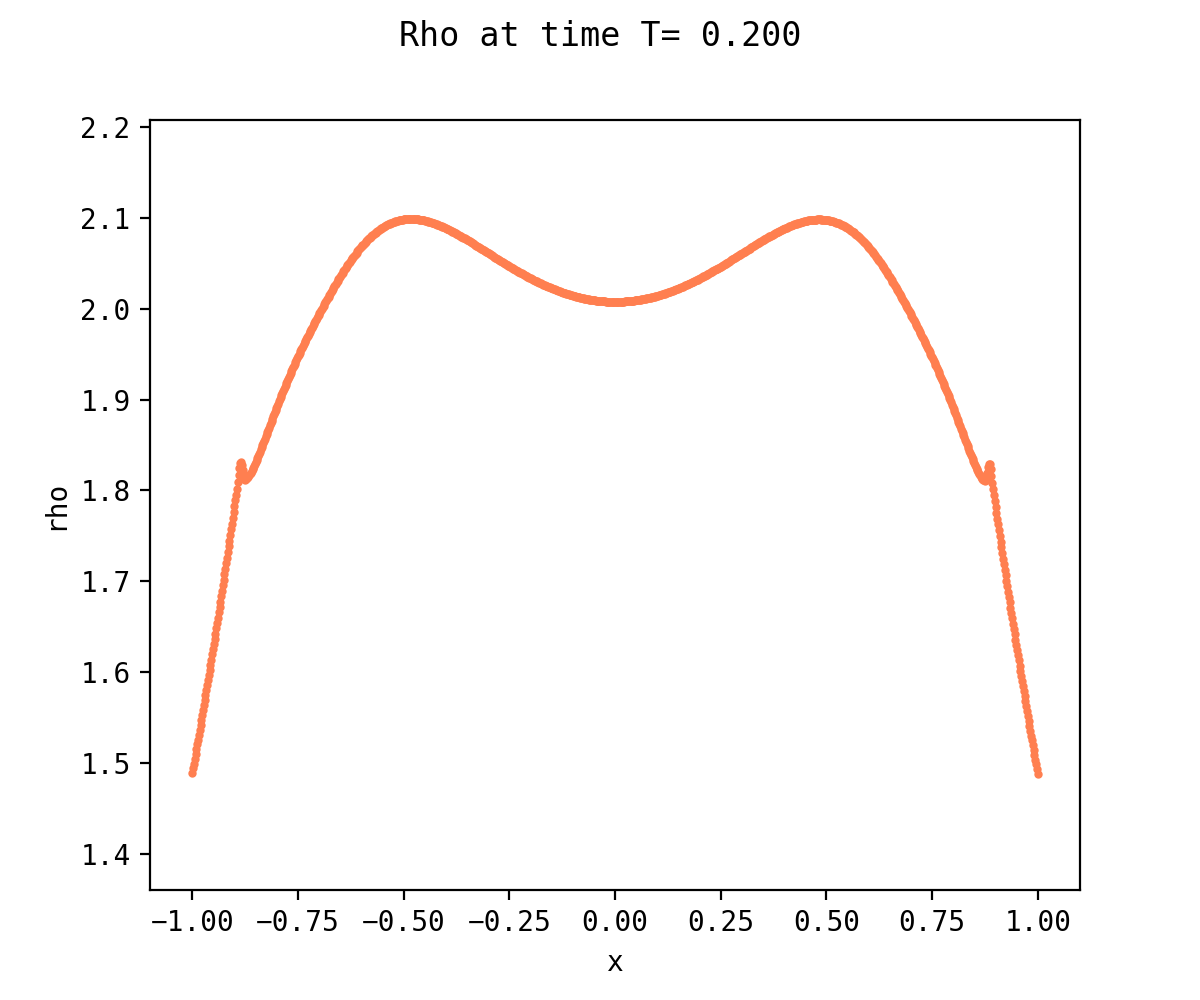
\includegraphics[height=\imh,width=\imw]{images/rhoT0p2.png}
		\caption{Density $\rho$}
		\label{subfig:compT02_rho}
	\end{subfigure}
	
	\begin{subfigure}{\textwidth}
		\centering
		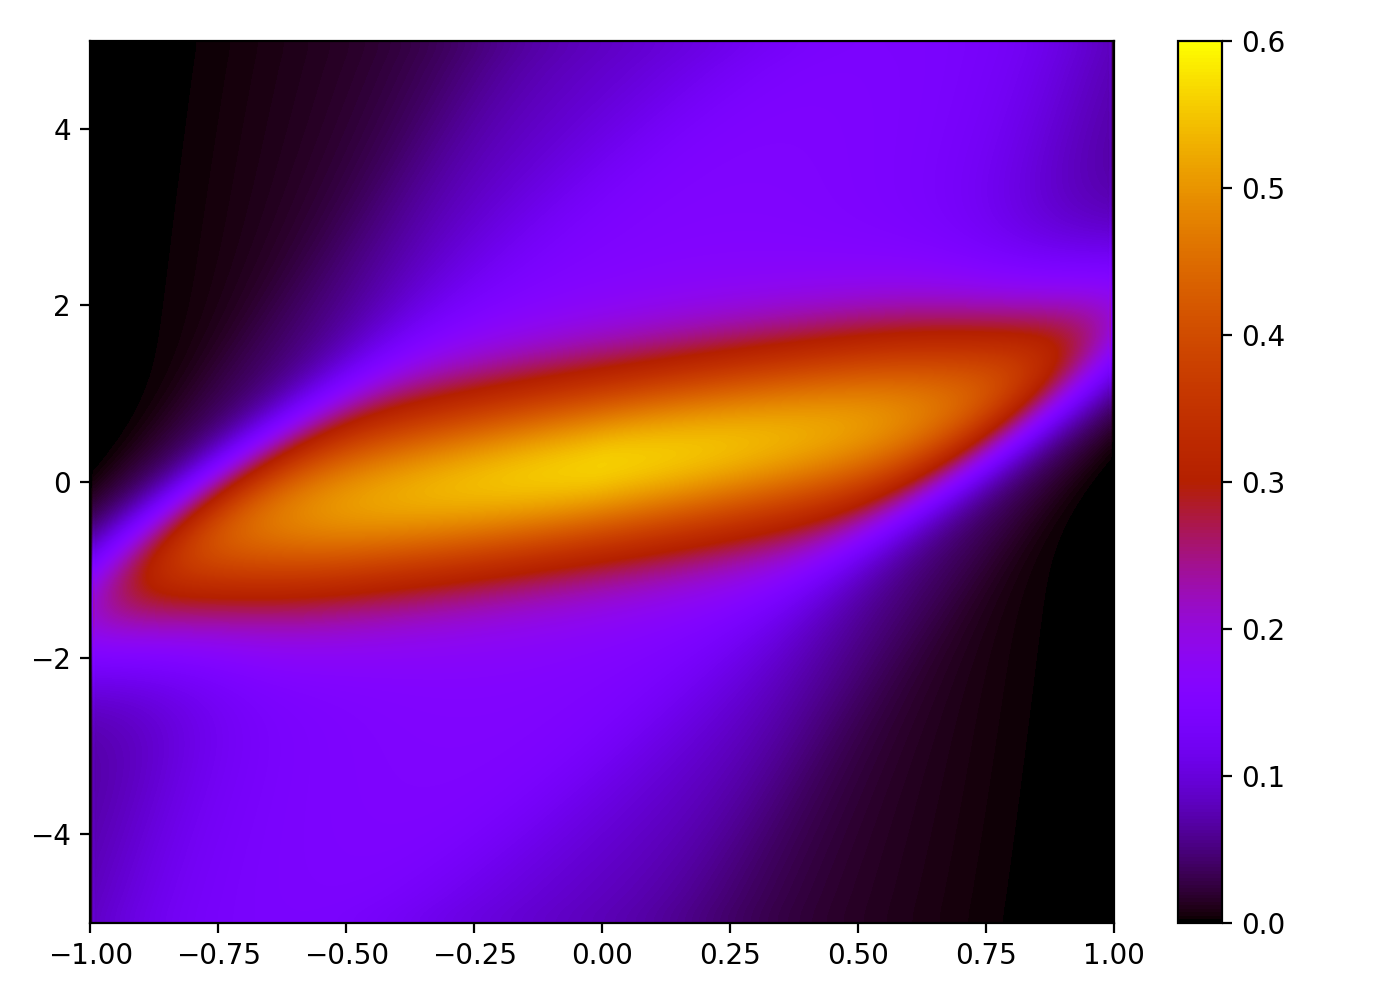
\includegraphics[height=\imh,width=\imw]{images/fiT0p2_FD.png}
		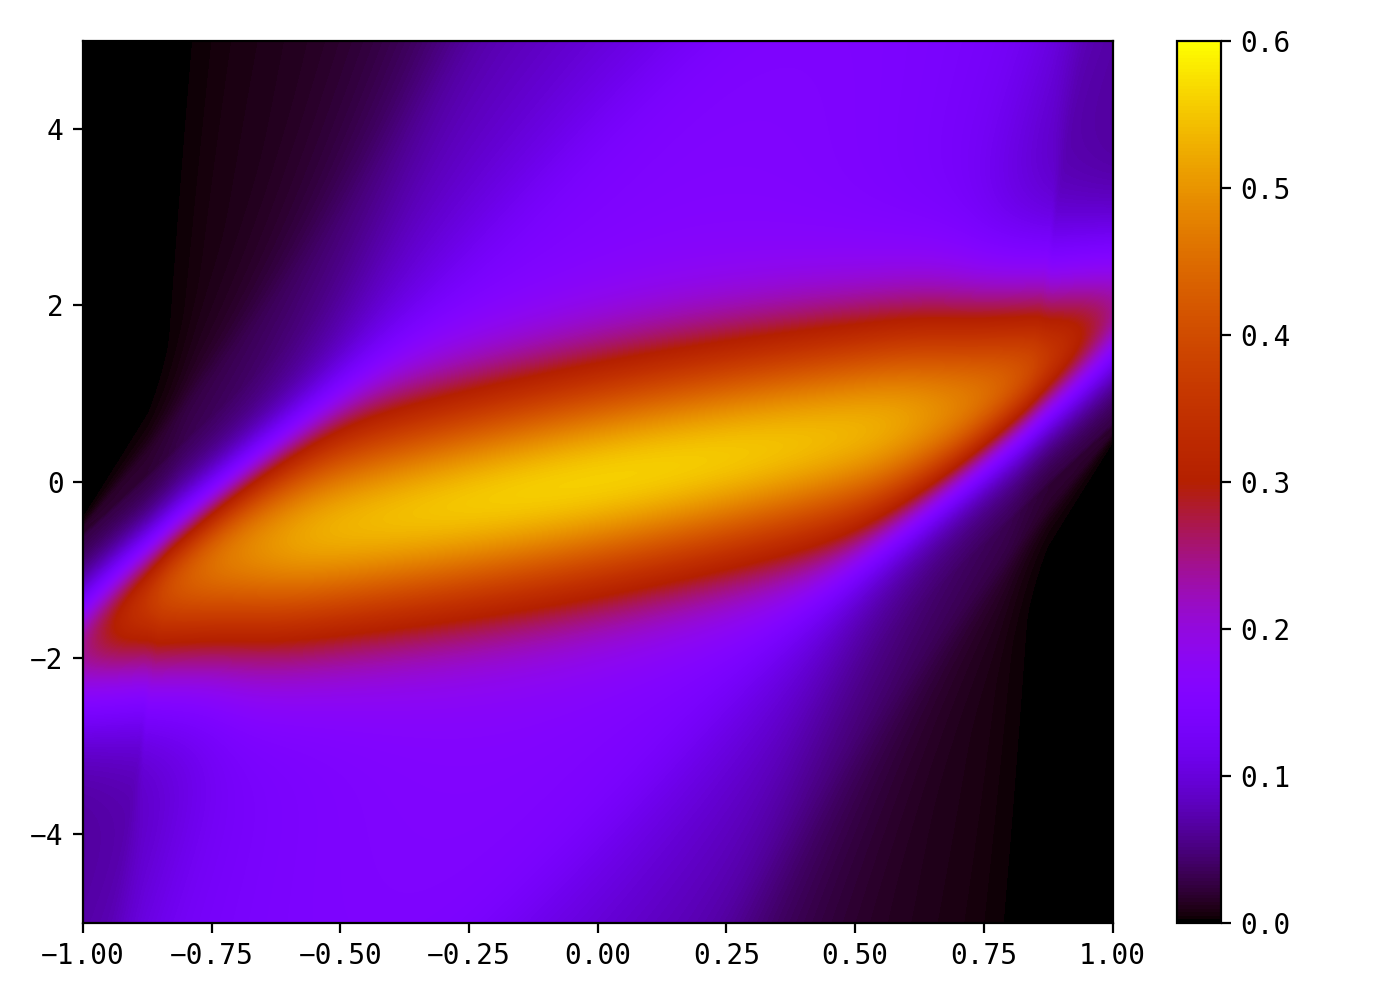
\includegraphics[height=\imh,width=\imw]{images/fiT0p2.png}
		\caption{Ion distribution function}
		\label{subfig:compT02_ion}
	\end{subfigure}
	\begin{subfigure}{\textwidth}
		\centering
		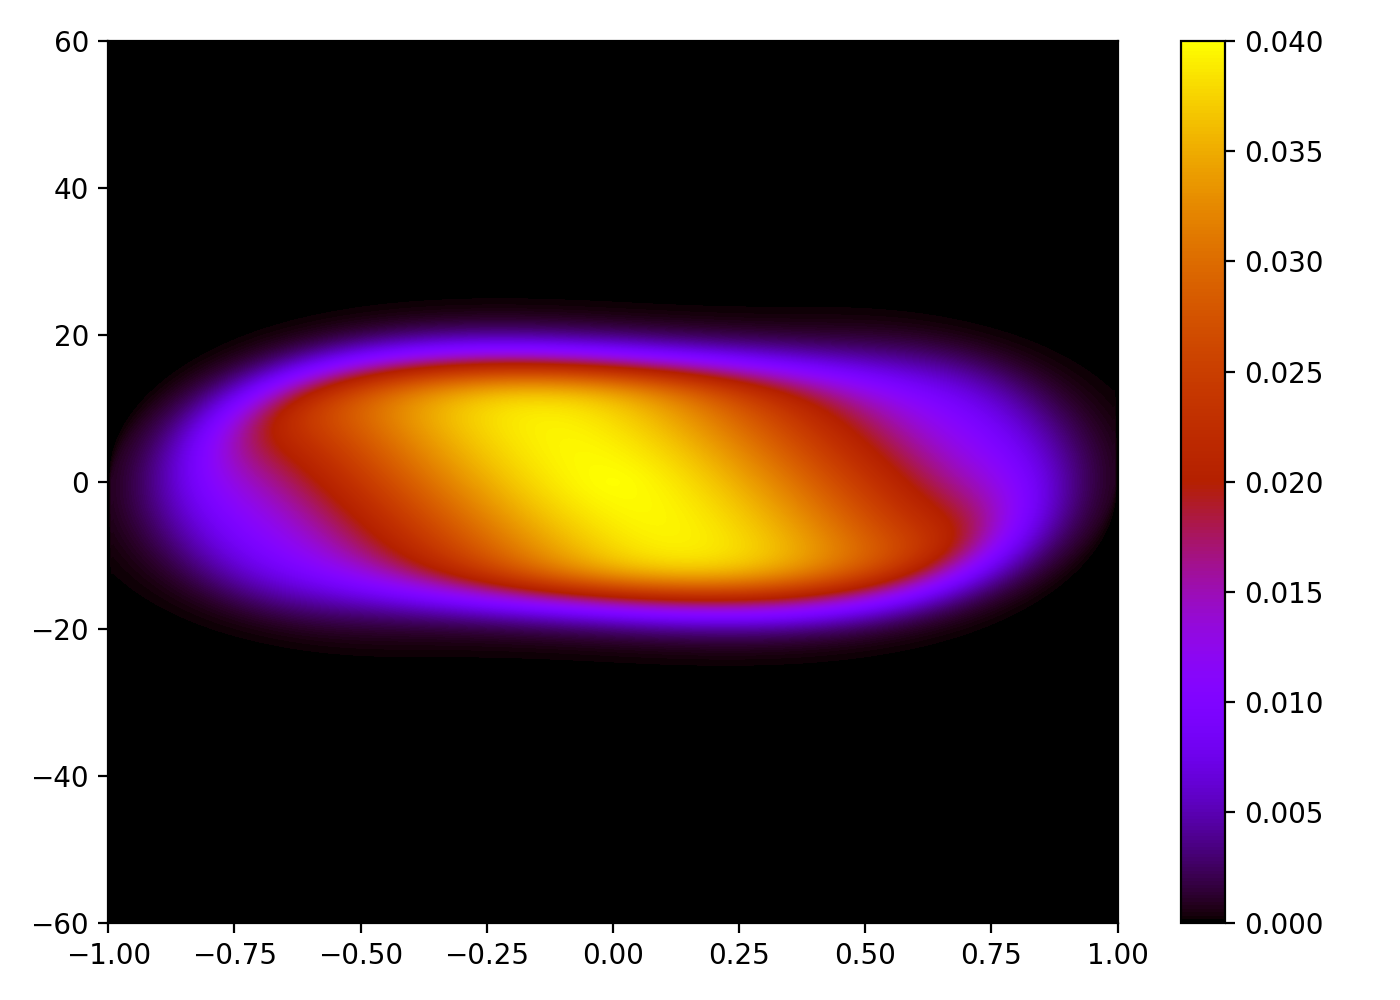
\includegraphics[height=\imh,width=\imw]{images/feT0p2_FD.png}
		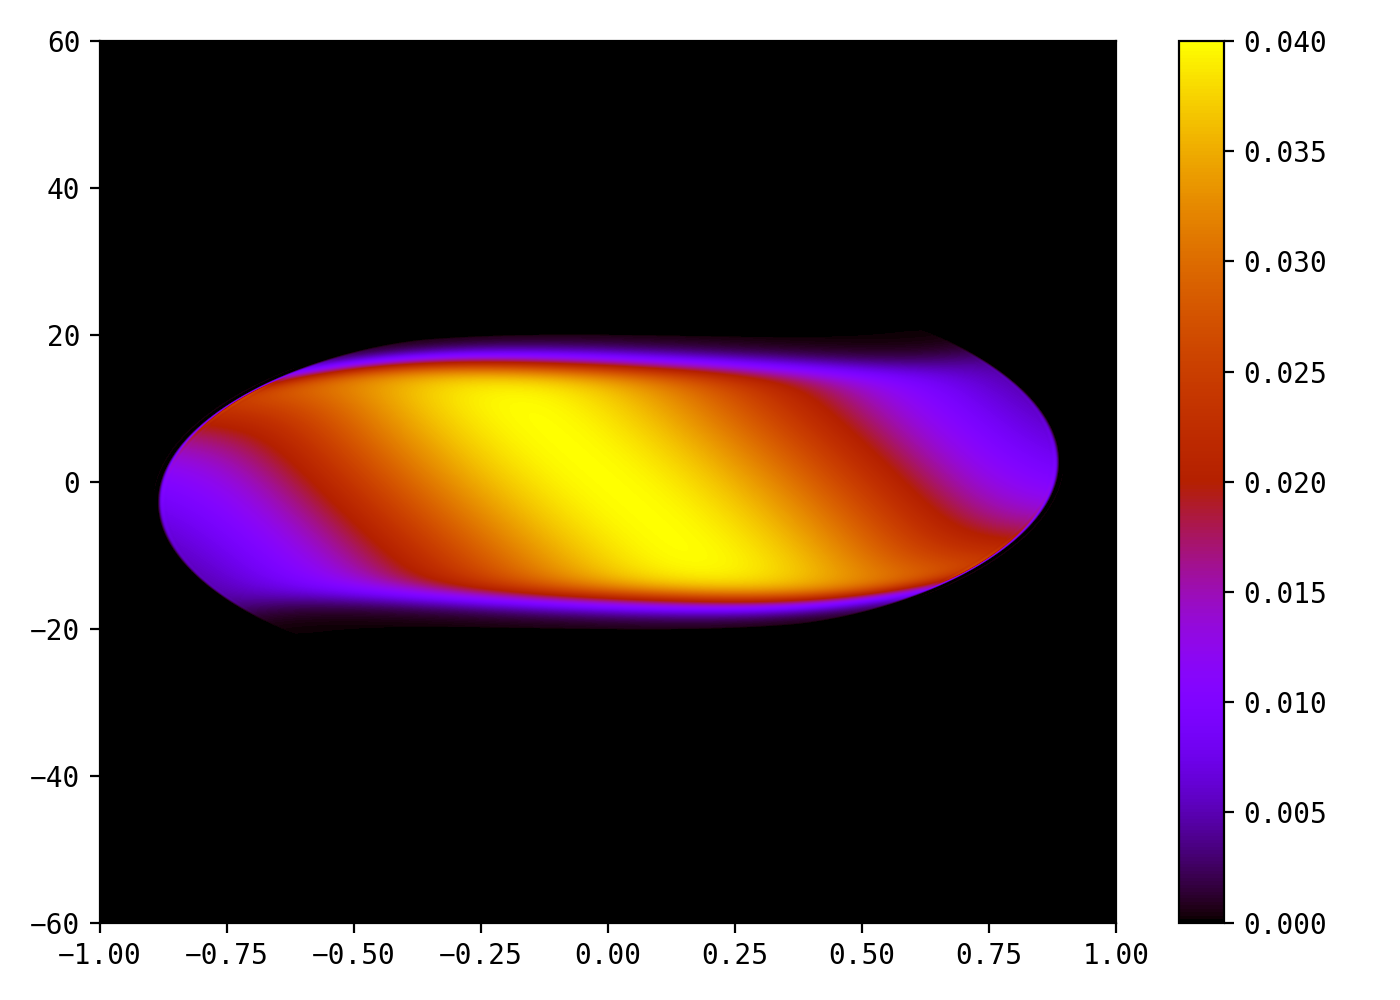
\includegraphics[height=\imh,width=\imw]{images/feT0p2.png}
		\caption{Electron distribution function}
		\label{subfig:compT02_electron}
	\end{subfigure}
	\caption{Comparison between finite differences (left) and semi-Lagrangian (right) at $T=0.2$. The Semi-Lagrangian code uses parameters of Run2.}
	\label{fig:compT02}
\end{figure}  

\begin{figure}
	\centering
	\newcommand{\rootSL}{../code_SL/}
%	\newcommand{\rootFD}{../../DynamicElectricSheath.jl/data/two_species/}
	\newcommand{\rootFD}{../temp_res_DF/}
	\newcommand{\dirSL}{run_comp_short_time_2sp_Nx1000_Nvi2001_Nve2001_Nt6250}
	\newcommand{\dirFD}{run_comp_short_time_2sp_Nx1000_Nv2000_Nt6250}
	
	\renewcommand{\imh}{0.24\textheight}
	\renewcommand{\imw}{0.45\linewidth}
	
	\begin{subfigure}{\textwidth}
		\centering
		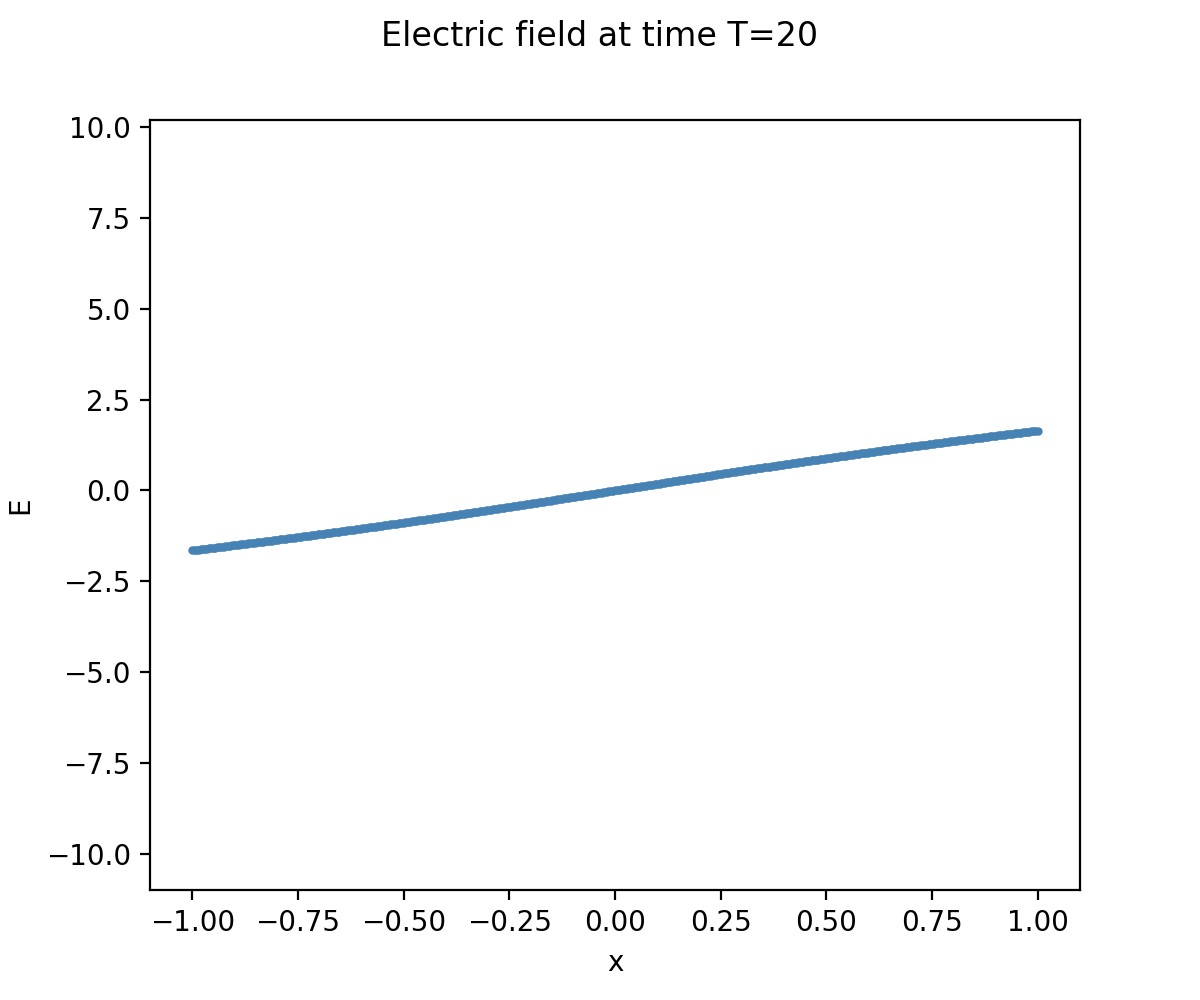
\includegraphics[height=\imh,width=\imw]{images/ET20_FD.png}
		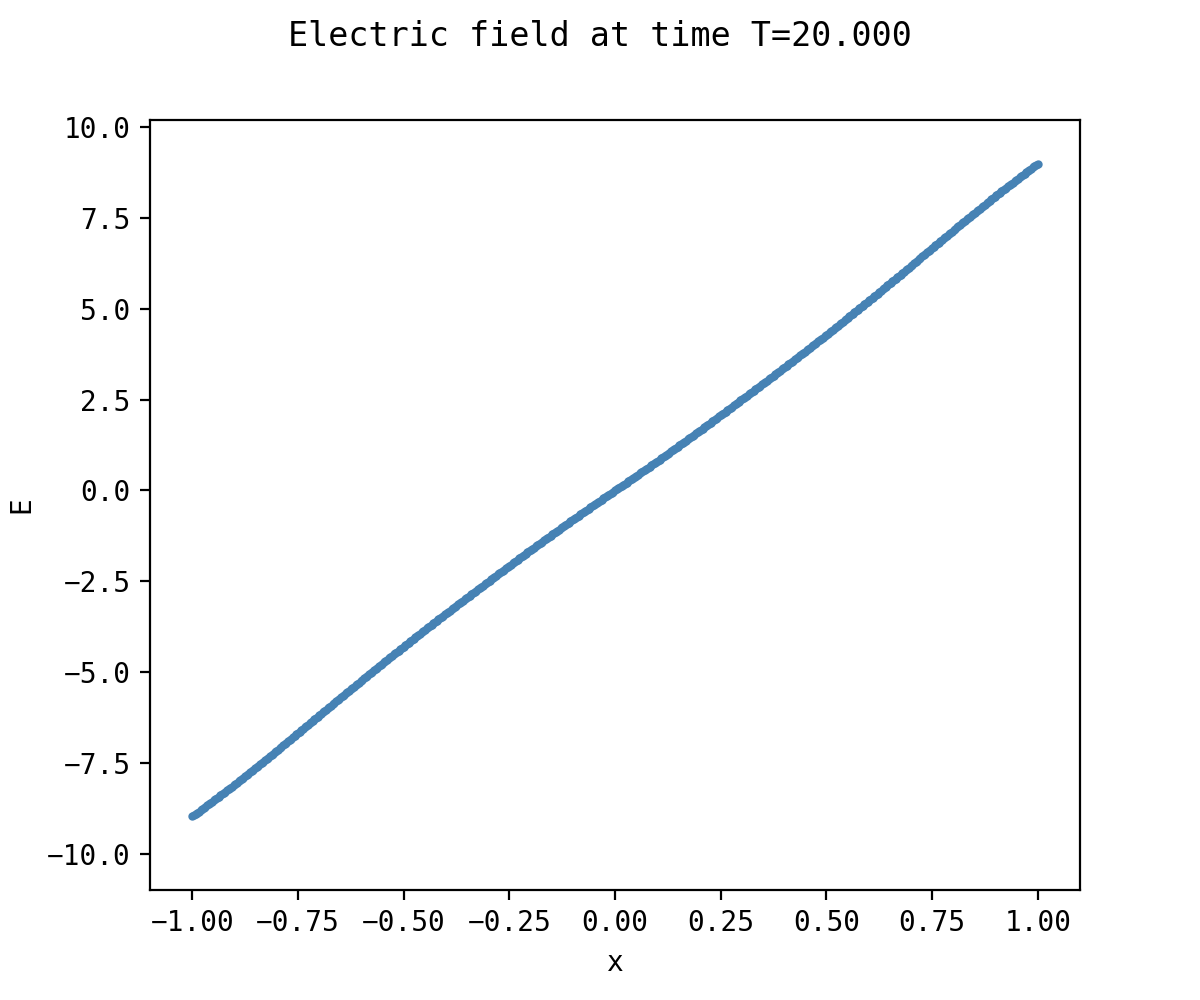
\includegraphics[height=\imh,width=\imw]{images/ET20_512.png}
		\caption{Electric field }
		\label{subfig:compT02_E}
	\end{subfigure}

	\begin{subfigure}{\textwidth}
		\centering
		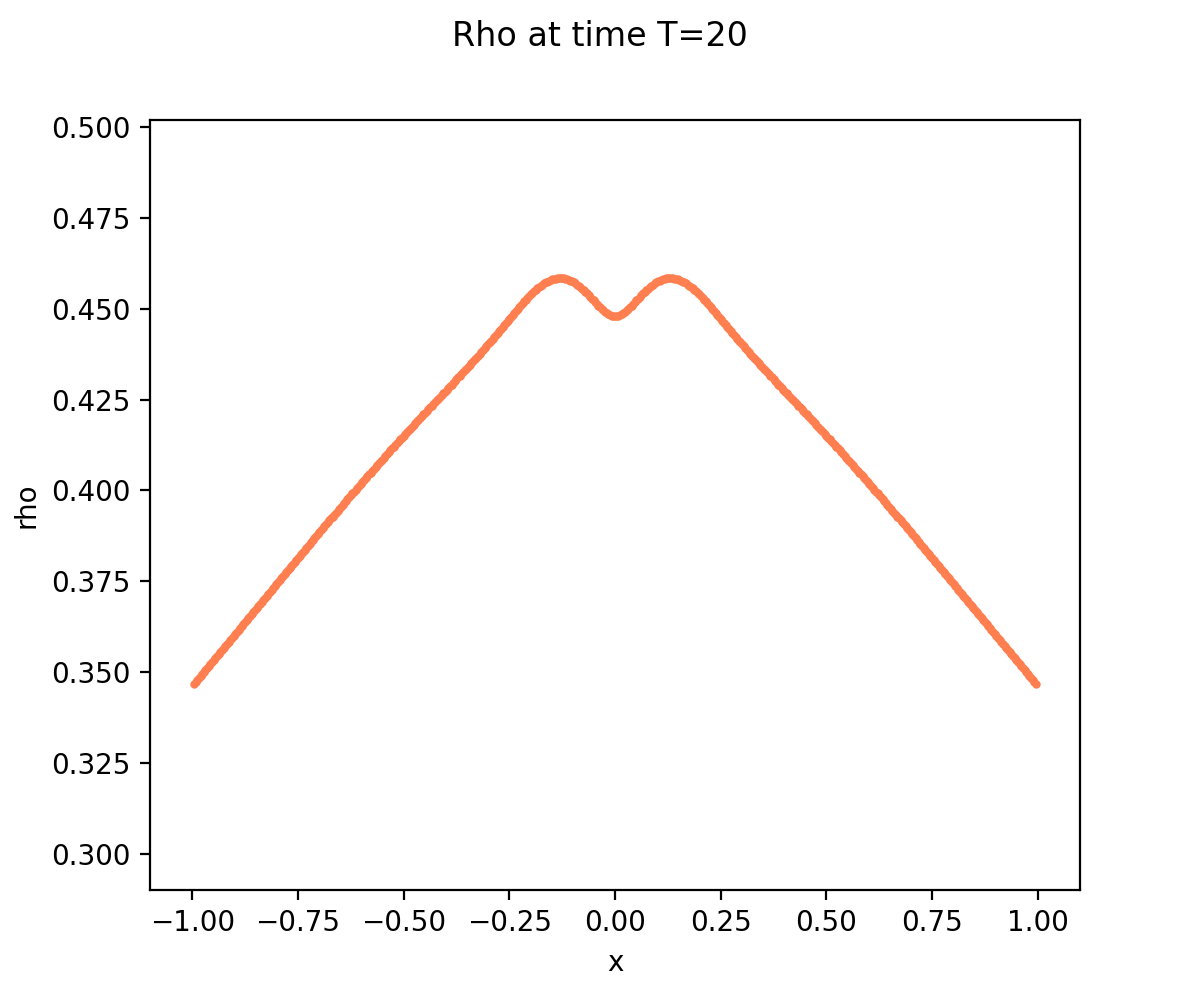
\includegraphics[height=\imh,width=\imw]{images/rhoT20_FD.png}
		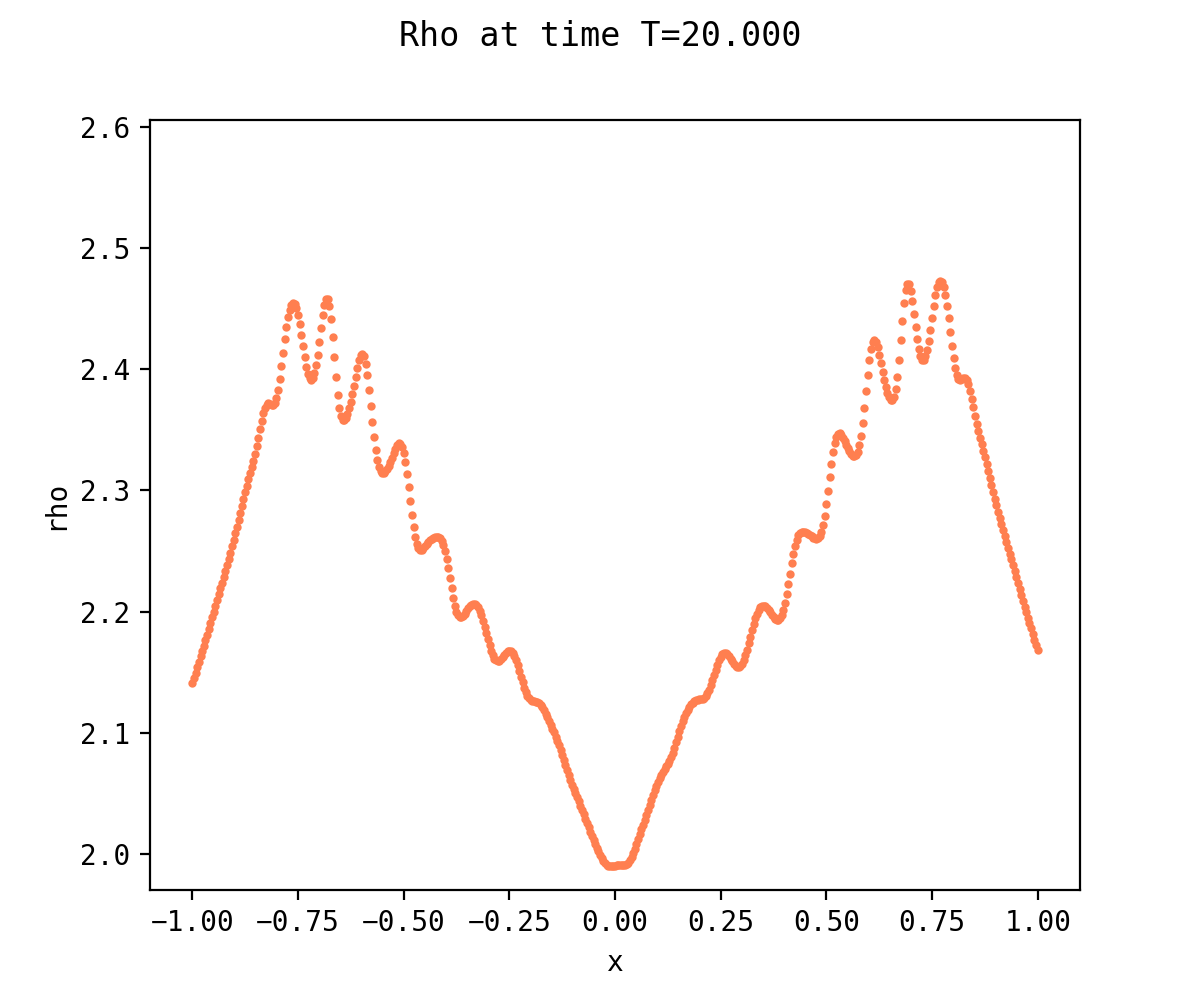
\includegraphics[height=\imh,width=\imw]{images/rhoT20_512.png}
		\caption{Density $\rho$}
		\label{subfig:compT02_rho}
	\end{subfigure}
	
	\begin{subfigure}{\textwidth}
		\centering
		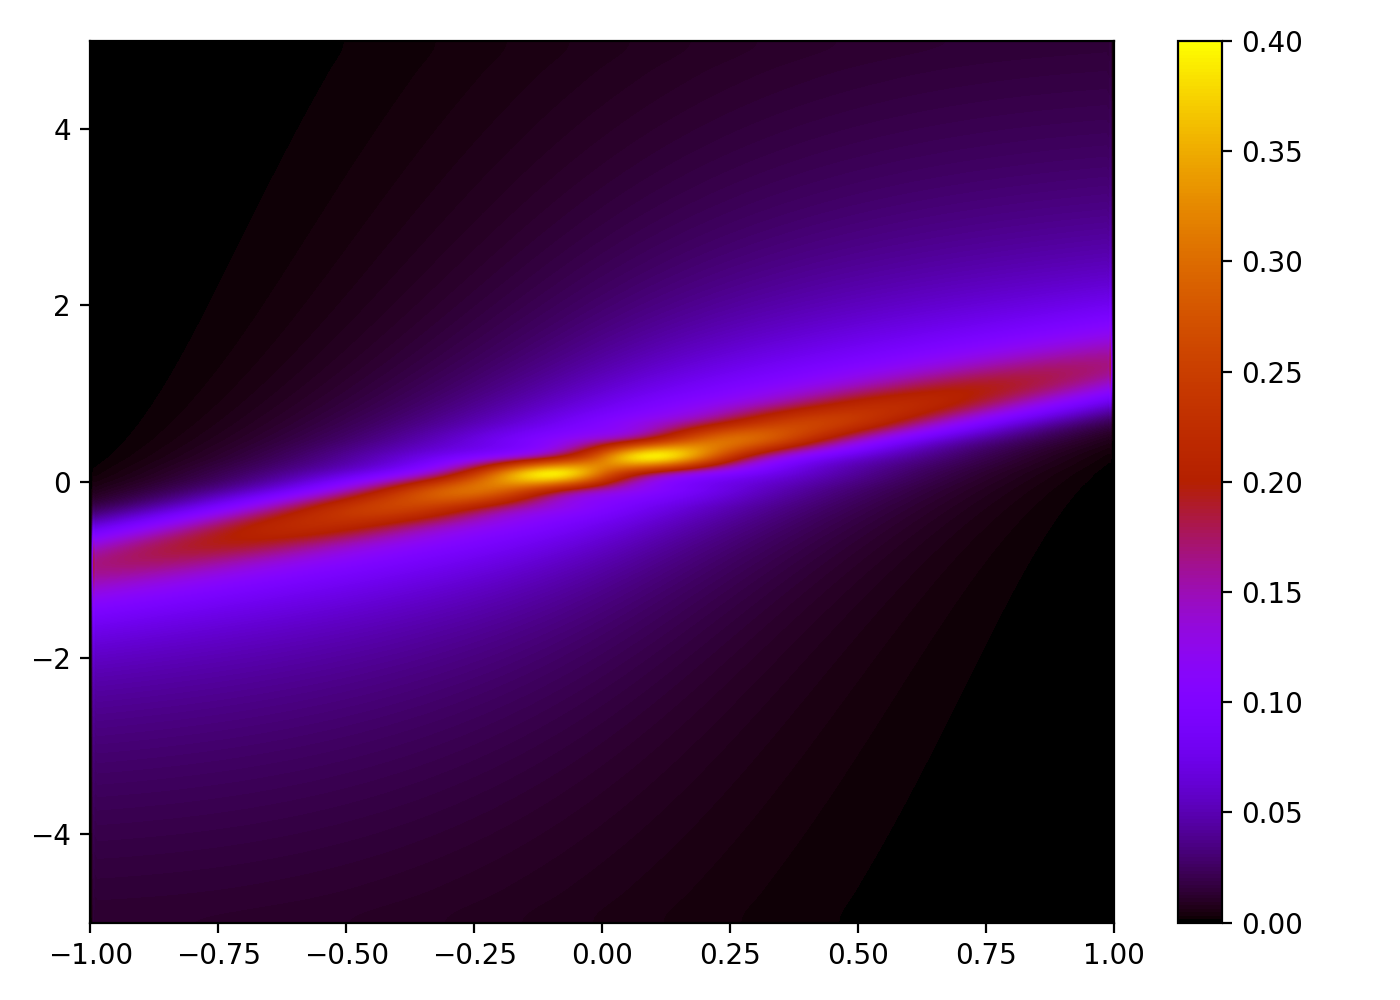
\includegraphics[height=\imh,width=\imw]{images/fiT20_FD.png}
		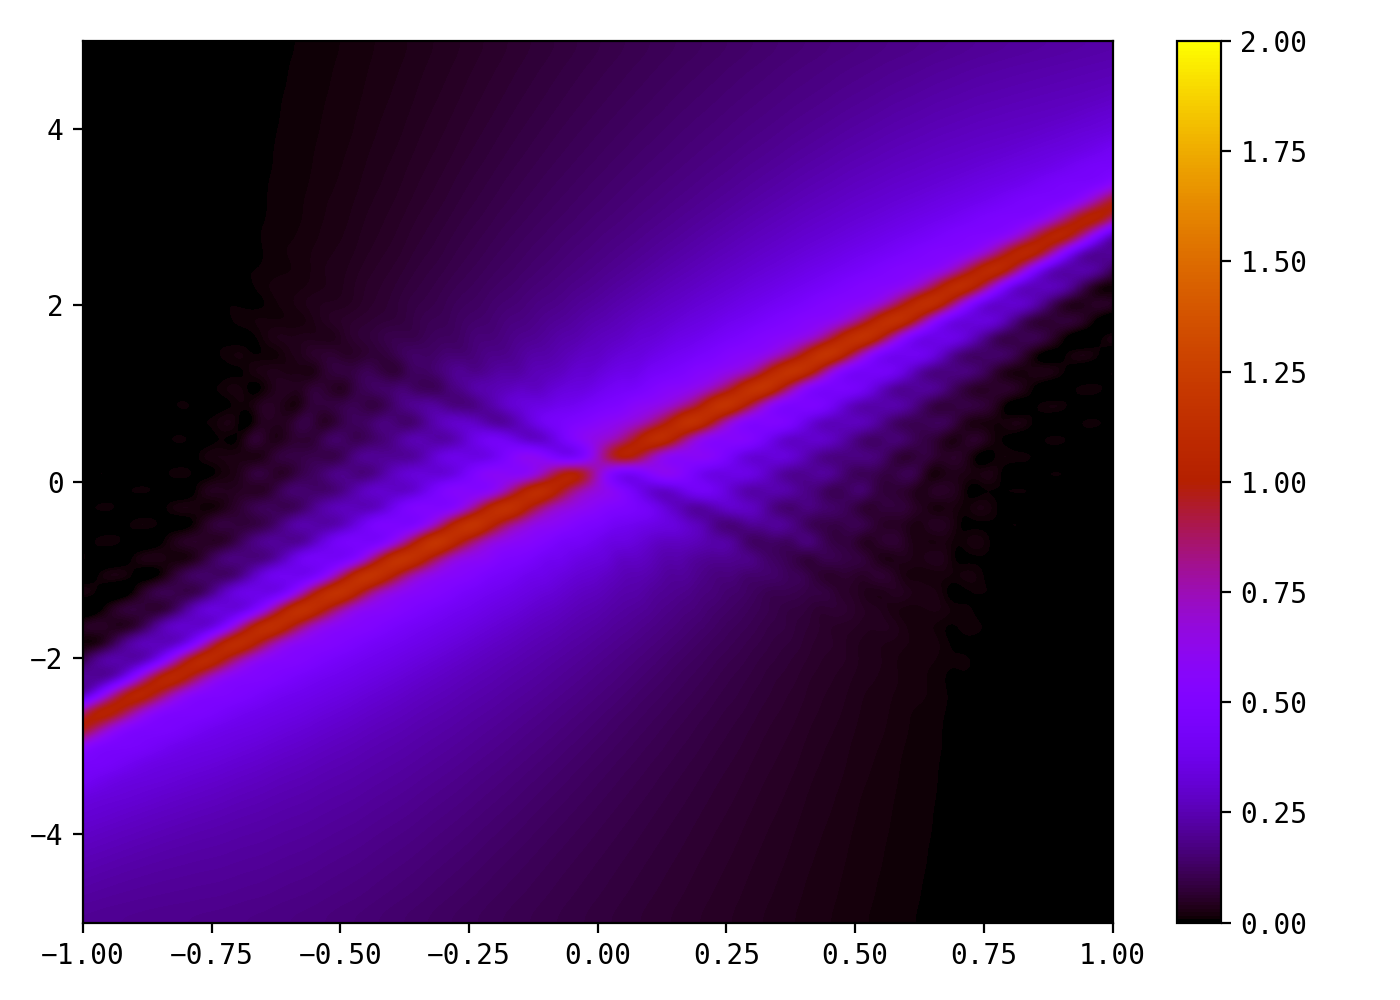
\includegraphics[height=\imh,width=\imw]{images/fiT20_512.png}
		\caption{Ion distribution function}
		\label{subfig:compT02_ion}
	\end{subfigure}
	\begin{subfigure}{\textwidth}
		\centering
		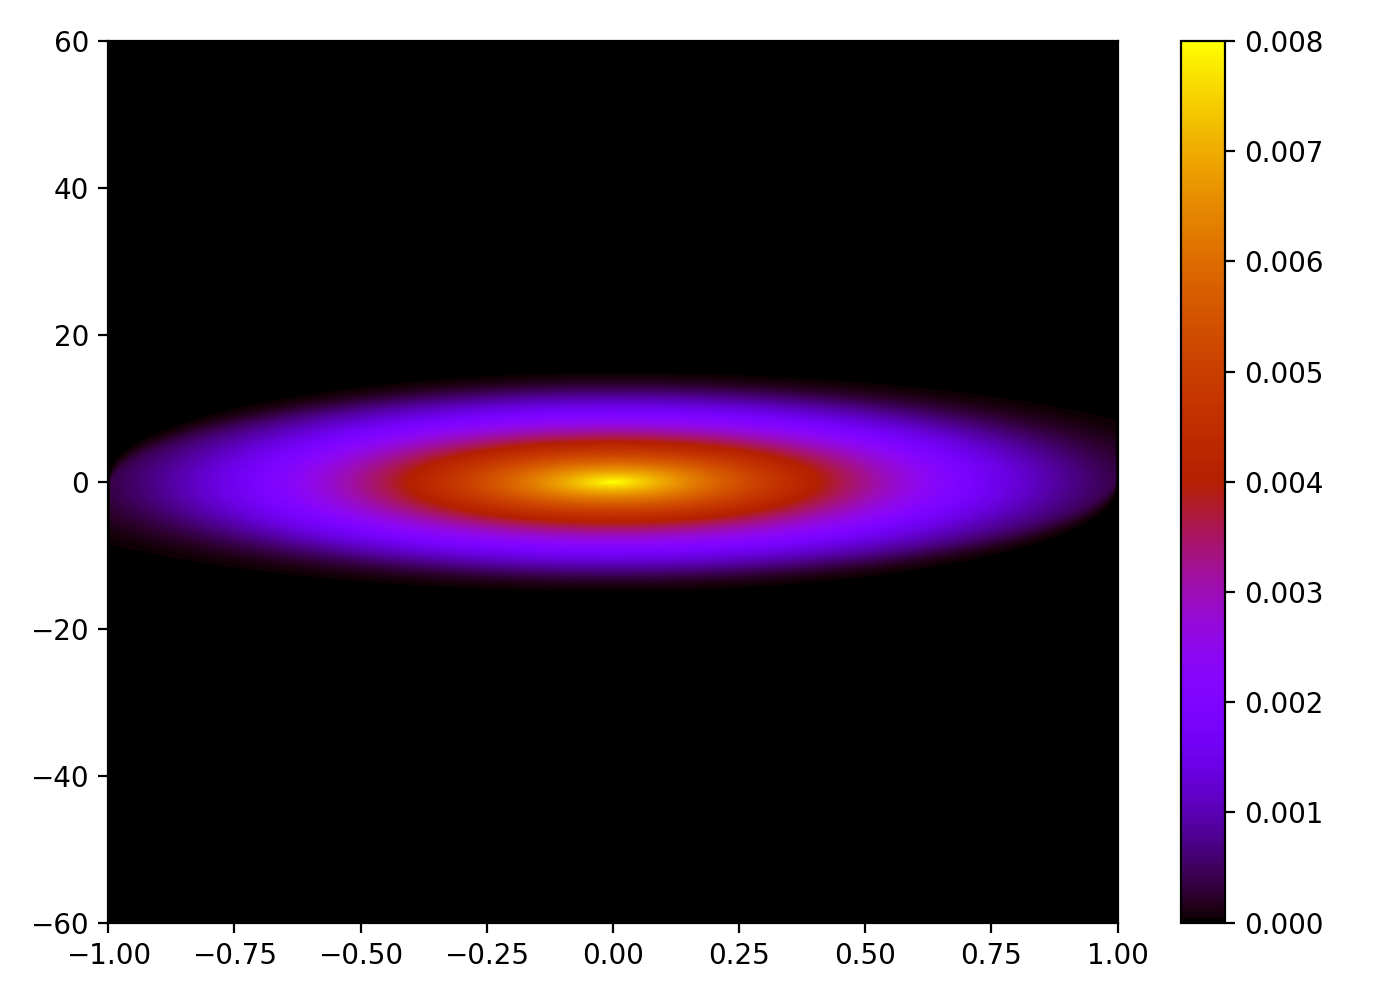
\includegraphics[height=\imh,width=\imw]{images/feT20_FD.png}
		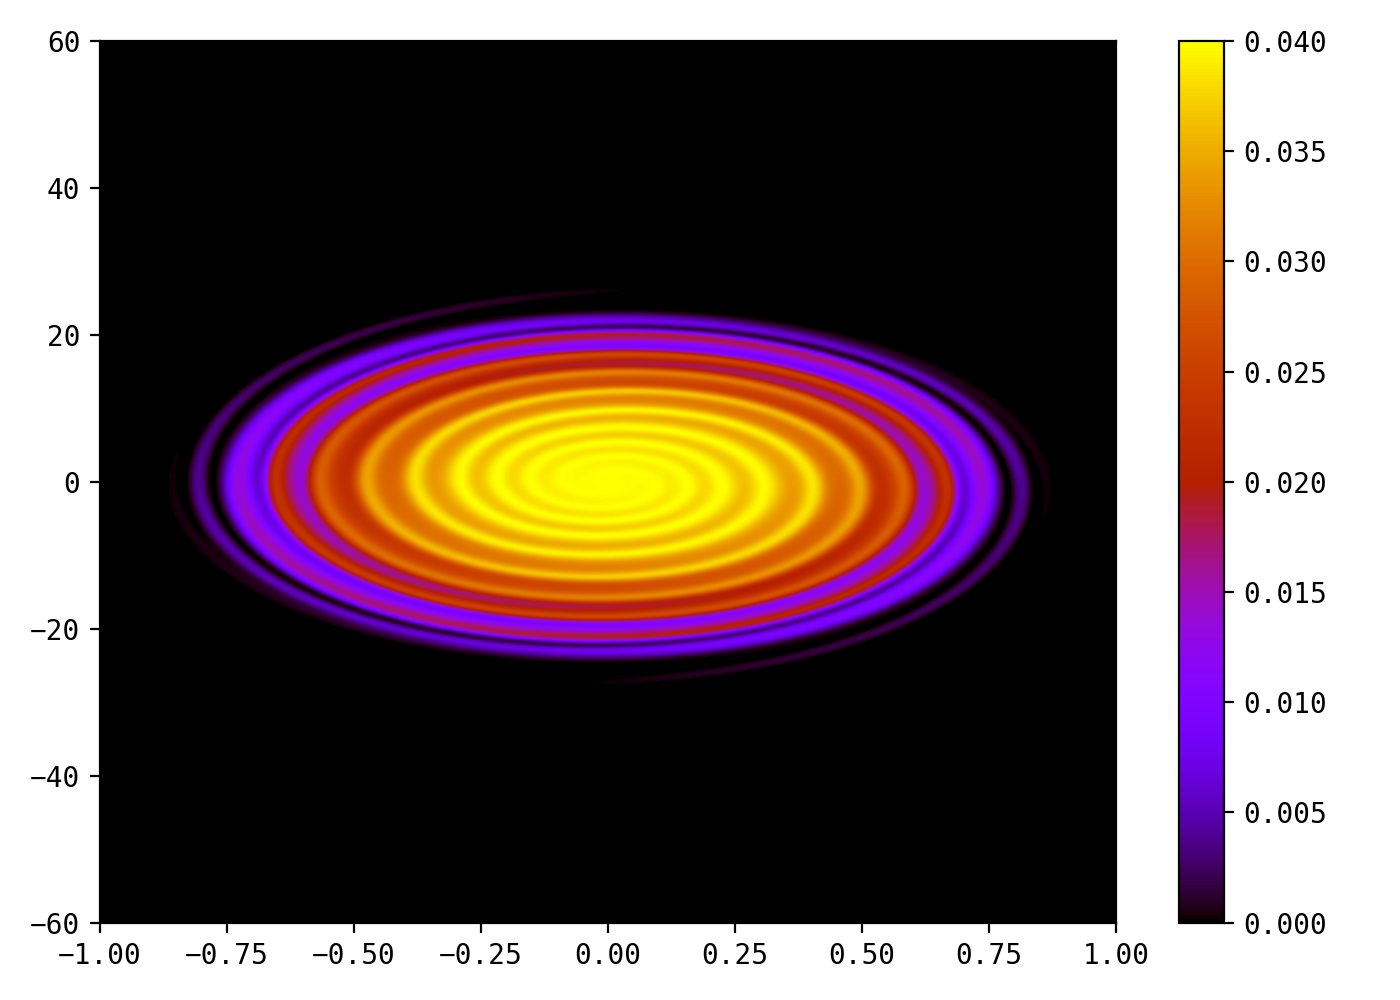
\includegraphics[height=\imh,width=\imw]{images/feT20_512.png}
		\caption{Electron distribution function}
		\label{subfig:compT02_electron}
	\end{subfigure}
	\caption{Comparison between finite differences (left) and semi-Lagrangian  (right) at $T=20$. The Semi-Lagrangian code uses parameters of Run0.
	%, with $N_x=512,\ N_{v_e}=N_{v_i}=513$ for both codes. %For the semi-Lagrangian code, we use $\Delta t=0.00025$, $[-60,60]$ for $v_e$ and  $[-50,50]$ for $v_i$. The ion density is zoomed for $v_i\in [-5,5]$
	}
	\label{fig:compT20}
\end{figure}  

%\begin{figure}
%	\centering
%	\newcommand{\rootSL}{../code_SL/}
%%	\newcommand{\rootFD}{../../DynamicElectricSheath.jl/data/two_species/}
%	\newcommand{\rootFD}{../temp_res_DF/}
%	\newcommand{\dirSL}{run_comp_long_time_2sp_Nx1000_Nvi2001_Nve2001_Nt100000}
%	\newcommand{\dirFD}{run_comp_long_time_2sp_Nx200_Nv400_Nt2500000}
%	
%	\renewcommand{\imh}{0.33\linewidth}
%	
%	\begin{subfigure}{\textwidth}
%		\centering
%		\includegraphics[height=\imh]{\rootFD\dirFD/comp_E_\dirSL.png}
%		\includegraphics[height=\imh]{\rootFD\dirFD/comp_rho_\dirSL.png}
%		\caption{Electric field (left) and density $\rho$ (right)}
%		\mysubcaption{The maximum of $\rho$ for the (DF) code is equal to 39.983965094090.}
%		\label{subfig:compT200_E_rho}
%	\end{subfigure}
%	
%	\begin{subfigure}{\textwidth}
%		\centering
%		\includegraphics[height=\imh]{\rootFD\dirFD/fi}
%		\includegraphics[height=\imh]{\rootSL\dirSL/python_diags/fi}
%		\caption{Ion density} 
%		\label{subfig:compT200_ion}
%	\end{subfigure}
%	\begin{subfigure}{\textwidth}
%		\centering
%		\includegraphics[height=\imh]{\rootFD\dirFD/fe}
%		\includegraphics[height=\imh]{\rootSL\dirSL/python_diags/fe}
%		\caption{Electron density}
%		\label{subfig:compT200_electron}
%	\end{subfigure}
%	\caption{Comparison between finite differences (left) and semi-Lagrangian (right) at $T=200$.}
%	\label{fig:compT200}
%\end{figure}  

%The behavior of the ion densition 
\begin{figure}
	\centering
	\newcommand{\rootSL}{../code_SL/}
%	\newcommand{\rootFD}{../../DynamicElectricSheath.jl/data/two_species/}
	\newcommand{\rootFD}{../temp_res_DF/}
	\newcommand{\dirSL}{run_comp_long_time_2sp_Nx1000_Nvi2001_Nve2001_Nt100000}
	\newcommand{\dirFD}{run_comp_long_time_2sp_Nx200_Nv400_Nt2500000}
	
	\renewcommand{\imh}{0.24\textheight}
	\renewcommand{\imw}{0.45\linewidth}
	
	\begin{subfigure}{\textwidth}
		\centering
		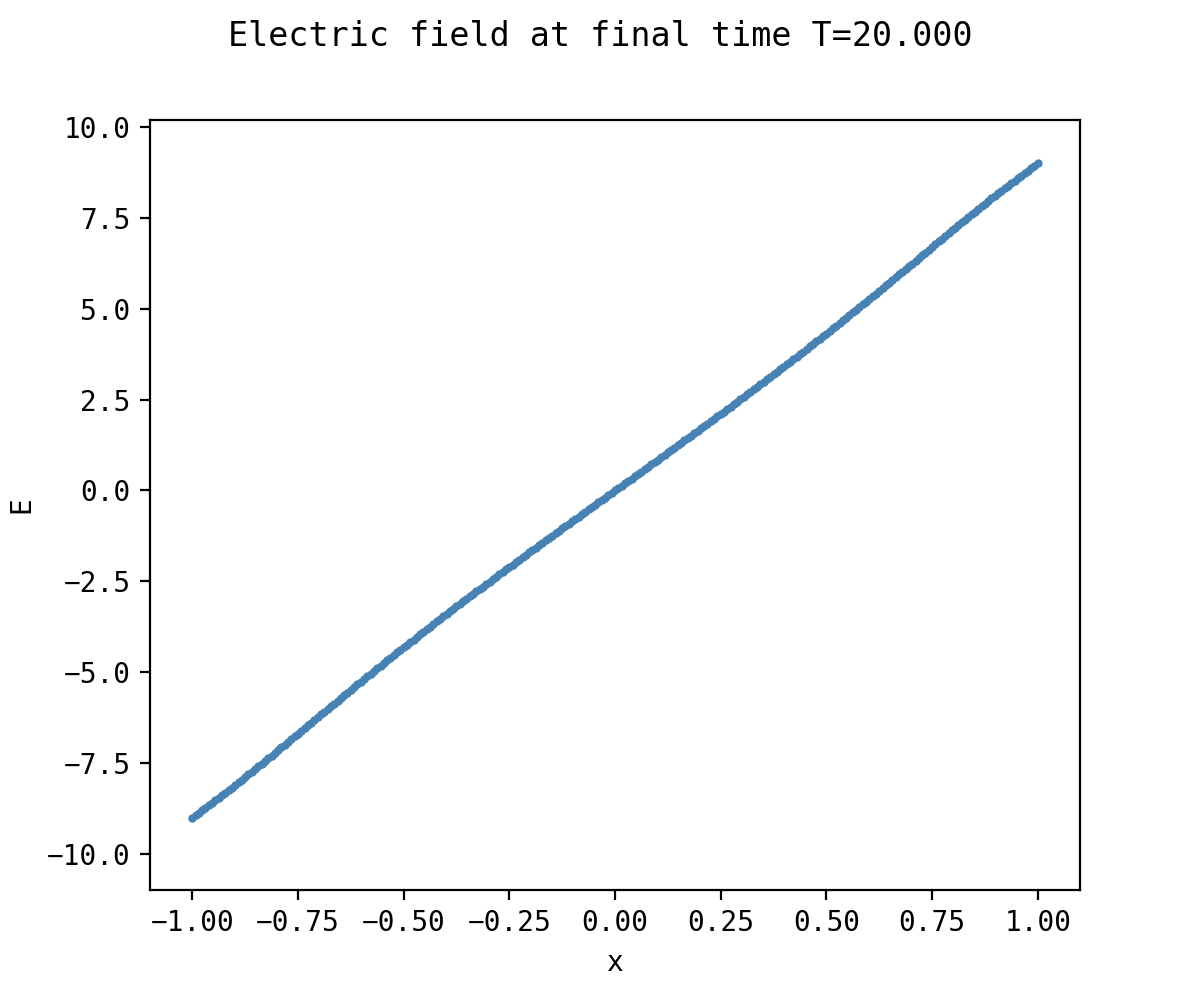
\includegraphics[height=\imh,width=\imw]{images/E_run5ab.png}
		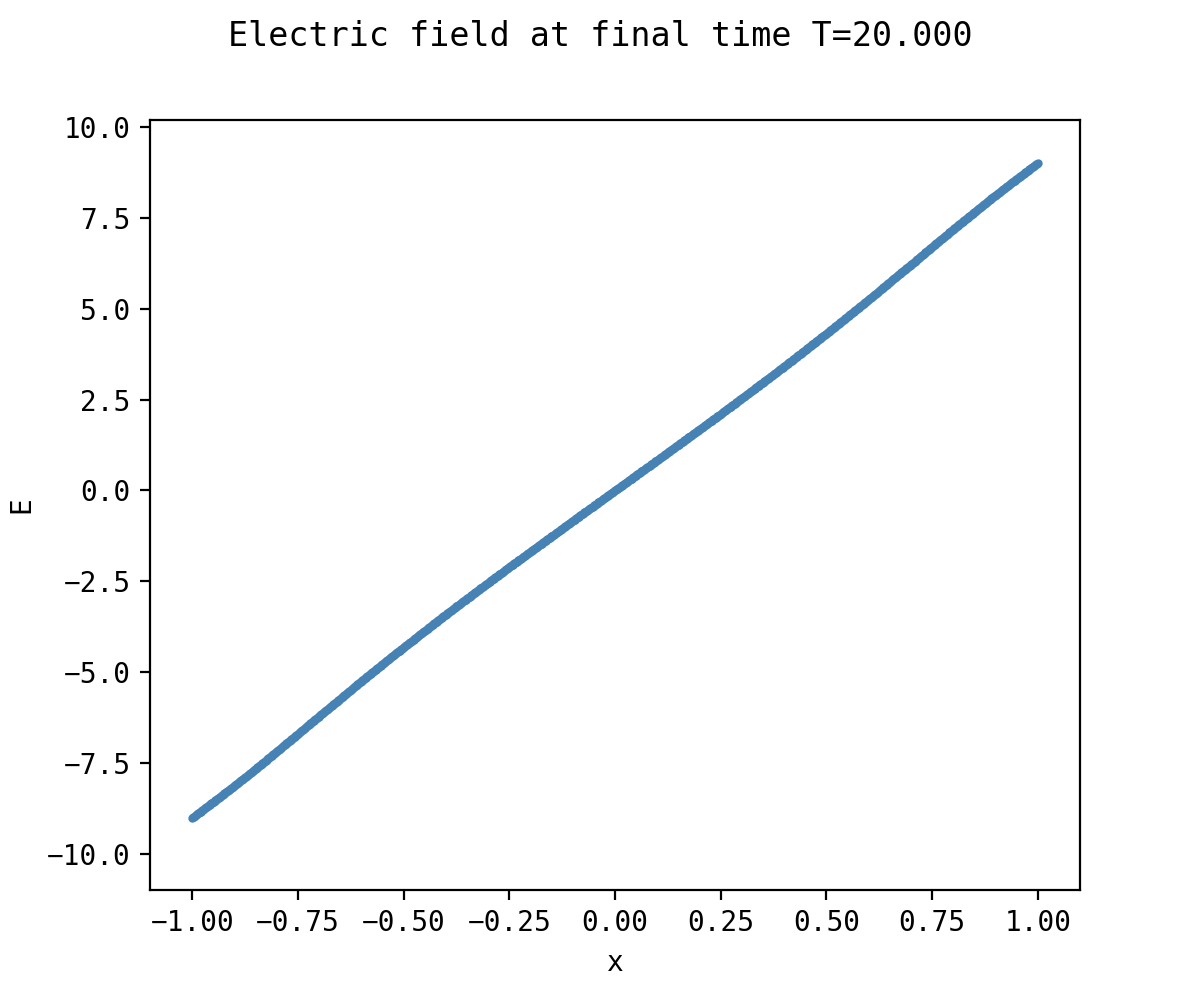
\includegraphics[height=\imh,width=\imw]{images/E_run5ac.png}
		\caption{Electric field}
		%\mysubcaption{The maximum of $\rho$ for the (DF) code is equal to 39.983965094090.}
		%\label{subfig:compT200_E_rho}
	\end{subfigure}
	\begin{subfigure}{\textwidth}
		\centering
		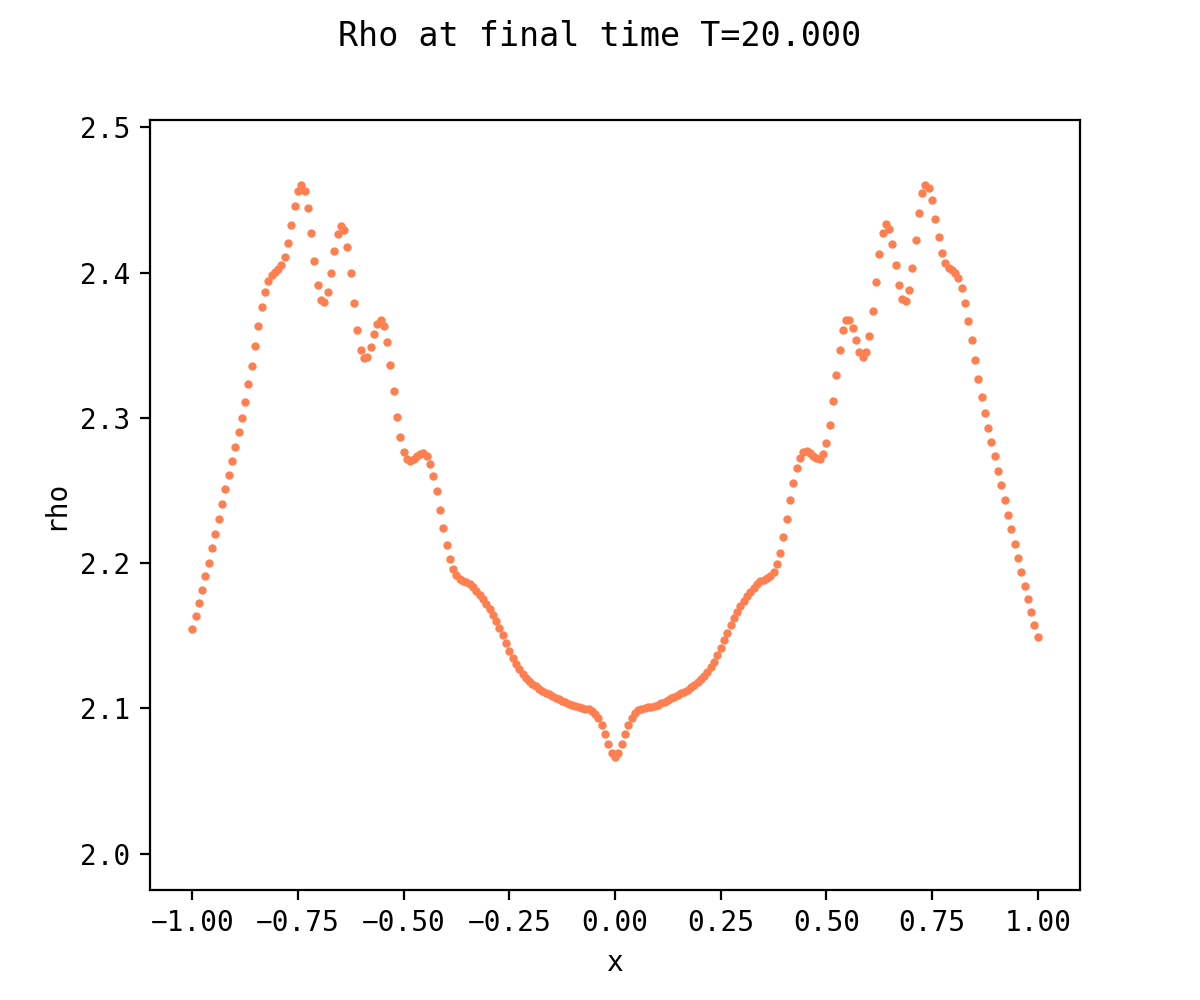
\includegraphics[height=\imh,width=\imw]{images/rho_run5ab.png}
		\includegraphics[height=\imh,width=\imw]{images/rho_run5ac.png}
		\caption{Density $\rho$}
		%\mysubcaption{The maximum of $\rho$ for the (DF) code is equal to 39.983965094090.}
		%\label{subfig:compT200_E_rho}
	\end{subfigure}
	
	\begin{subfigure}{\textwidth}
		\centering
		\includegraphics[height=\imh,width=\imw]{images/fi_run5ab.png}
		\includegraphics[height=\imh,width=\imw]{images/fi_run5ac.png}
		\caption{Ion distribution function} 
		%\label{subfig:compT200_ion}
	\end{subfigure}
	\begin{subfigure}{\textwidth}
		\centering
		\includegraphics[height=\imh,width=\imw]{images/fe_run5ab.png}
		\includegraphics[height=\imh,width=\imw]{images/fe_run5ac.png}
		\caption{Electron distribution function}
		%\label{subfig:compT200_electron}
	\end{subfigure}
	\caption{Comparison of semi-Lagrangian codes: parameter of Run1 (left) and parameters of Run2 (right).}
	%for different discretizations. Run1:  $N_x=256,\ N_{v_i}=2049$ (left); Run2: $N_x=1024,\ N_{v_i}=4097$ (right) at $T=20$.
	%Other numerical parameters are $N_{v_e}=8193$ and $\Delta t = 0.00025$. We have used $[-60,60]$ for $v_e$ and  $[-50,50]$ for $v_i$.
	%The ion density is zoomed for $v_i\in [-5,5]$
	%}
	\label{fig:comp_phasespace}
\end{figure}  

\begin{figure}
	\centering
	\newcommand{\rootSL}{../code_SL/}
%	\newcommand{\rootFD}{../../DynamicElectricSheath.jl/data/two_species/}
	\newcommand{\rootFD}{../temp_res_DF/}
	\newcommand{\dirSL}{run_comp_long_time_2sp_Nx1000_Nvi2001_Nve2001_Nt100000}
	\newcommand{\dirFD}{run_comp_long_time_2sp_Nx200_Nv400_Nt2500000}
	
	\renewcommand{\imh}{0.24\textheight}
	\renewcommand{\imw}{0.45\linewidth}
	
	\begin{subfigure}{\textwidth}
		\centering
		\includegraphics[height=\imh,width=0.3\linewidth]{images/rhoT1.png}
		\includegraphics[height=\imh,width=0.3\linewidth]{images/feT1.png}
		\includegraphics[height=\imh,width=0.3\linewidth]{images/feT1_run_job2.png}
		\caption{$T=1$}
		%\mysubcaption{The maximum of $\rho$ for the (DF) code is equal to 39.983965094090.}
		%\label{subfig:compT200_E_rho}
	\end{subfigure}

	\begin{subfigure}{\textwidth}
		\centering
		\includegraphics[height=\imh,width=0.3\linewidth]{images/rhoT2.png}
		\includegraphics[height=\imh,width=0.3\linewidth]{images/feT2.png}
		\includegraphics[height=\imh,width=0.3\linewidth]{images/feT2_run_job2.png}
		\caption{$T=2$}
		%\mysubcaption{The maximum of $\rho$ for the (DF) code is equal to 39.983965094090.}
		%\label{subfig:compT200_E_rho}
	\end{subfigure}

	\begin{subfigure}{\textwidth}
		\centering
		\includegraphics[height=\imh,width=0.3\linewidth]{images/rhoT5.png}
		\includegraphics[height=\imh,width=0.3\linewidth]{images/feT5.png}
		\includegraphics[height=\imh,width=0.3\linewidth]{images/feT5_run_job2.png}
		\caption{$T=5$}
		%\mysubcaption{The maximum of $\rho$ for the (DF) code is equal to 39.983965094090.}
		%\label{subfig:compT200_E_rho}
	\end{subfigure}

	\begin{subfigure}{\textwidth}
		\centering
		\includegraphics[height=\imh,width=0.3\linewidth]{images/rhoT10.png}
		\includegraphics[height=\imh,width=0.3\linewidth]{images/feT10.png}
		\includegraphics[height=\imh,width=0.3\linewidth]{images/feT10_run_job2.png}
		\caption{$T=10$}
		%\mysubcaption{The maximum of $\rho$ for the (DF) code is equal to 39.983965094090.}
		%\label{subfig:compT200_E_rho}
	\end{subfigure}


	\caption{Density $\rho$ (left) and electron distribution function (middle and right) for time $T\in \{1,2,5,10\}$; 
	 The Semi-Lagrangian code is used with parameters of Run2 (left, middle) and of Run3 (right).
	%Run2; electron distribution function is also given, by changing $\Delta t$ to $0.000025$ (right)
	}
	\label{fig:comp_temps}
\end{figure}  

\begin{figure}
	\centering
	\newcommand{\rootSL}{../code_SL/}
%	\newcommand{\rootFD}{../../DynamicElectricSheath.jl/data/two_species/}
	\newcommand{\rootFD}{../temp_res_DF/}
	\newcommand{\dirSL}{run_comp_long_time_2sp_Nx1000_Nvi2001_Nve2001_Nt100000}
	\newcommand{\dirFD}{run_comp_long_time_2sp_Nx200_Nv400_Nt2500000}
	
	\renewcommand{\imh}{0.24\textheight}
	\renewcommand{\imw}{0.45\linewidth}
	
%	\begin{subfigure}{\textwidth}
%		\centering
%		\includegraphics[height=\imh,width=0.3\linewidth]{images/rhoT10_run5u.png}
%		\includegraphics[height=\imh,width=0.3\linewidth]{images/rhoT10_run5v.png}
%		\includegraphics[height=\imh,width=0.3\linewidth]{images/rhoT10_run5w.png}
%		\caption{$T=1$}
%		%\mysubcaption{The maximum of $\rho$ for the (DF) code is equal to 39.983965094090.}
%		%\label{subfig:compT200_E_rho}
%	\end{subfigure}

	\begin{subfigure}{\textwidth}
		\centering
		\includegraphics[height=\imh,width=0.45\linewidth]{images/rhoT5_run5af.png}
		\includegraphics[height=\imh,width=0.45\linewidth]{images/rhoT5_run5h.png}
		\caption{$\rho$ for $\Delta t=0.025$. $N_x=256, N_{v_e}=N_{v_i}=1023$ (left): $N_x=4096  , N_{v_e}=8193,\ N_{v_i}=16385$ (right)}
		%\mysubcaption{The maximum of $\rho$ for the (DF) code is equal to 39.983965094090.}
		%\label{subfig:compT200_E_rho}
	\end{subfigure}

	\begin{subfigure}{\textwidth}
		\centering
		\includegraphics[height=\imh,width=0.45\linewidth]{images/feT5_run5af.png}
		\includegraphics[height=\imh,width=0.45\linewidth]{images/feT5_run5h.png}
		\caption{$f_e$ for $\Delta t=0.025$. $N_x=256, N_{v_e}=N_{v_i}=1023$ (left): $N_x=4096  , N_{v_e}=8193,\ N_{v_i}=16385$ (right)}
		%\mysubcaption{The maximum of $\rho$ for the (DF) code is equal to 39.983965094090.}
		%\label{subfig:compT200_E_rho}
	\end{subfigure}
	\begin{subfigure}{\textwidth}
		\centering
		\includegraphics[height=\imh,width=0.45\linewidth]{images/rhoT5_run5n.png}
		\includegraphics[height=\imh,width=0.45\linewidth]{images/rhoT5_run5z.png}
		\caption{$\rho$ for $\Delta t=0.0025$. $N_x=256, N_{v_e}=N_{v_i}=1023$ (left): $N_x=512  , N_{v_e}=N_{v_i} = 8193$ (right)}
		%\mysubcaption{The maximum of $\rho$ for the (DF) code is equal to 39.983965094090.}
		%\label{subfig:compT200_E_rho}
	\end{subfigure}


	\begin{subfigure}{\textwidth}
		\centering
		\includegraphics[height=\imh,width=0.45\linewidth]{images/feT5_run5n.png}
		\includegraphics[height=\imh,width=0.45\linewidth]{images/feT5_run5z.png}
		\caption{$\rho$ for $\Delta t=0.0025$. $N_x=256, N_{v_e}=N_{v_i}=1023$ (left): $N_x=512  , N_{v_e}=N_{v_i} = 8193$ (right)}
		%\mysubcaption{The maximum of $\rho$ for the (DF) code is equal to 39.983965094090.}
		%\label{subfig:compT200_E_rho}
	\end{subfigure}

%	\begin{subfigure}{\textwidth}
%		\centering
%		\includegraphics[height=\imh,width=0.2\linewidth]{images/rhoT5_run5n.png}
%		\includegraphics[height=\imh,width=0.2\linewidth]{images/rhoT5_run5z.png}
%		\includegraphics[height=\imh,width=0.2\linewidth]{images/feT5_run5n.png}
%		\includegraphics[height=\imh,width=0.2\linewidth]{images/feT5_run5z.png}
%		\caption{$T=5$}
%		%\mysubcaption{The maximum of $\rho$ for the (DF) code is equal to 39.983965094090.}
%		%\label{subfig:compT200_E_rho}
%	\end{subfigure}


	\caption{Density $\rho$ and electron distribution function$f_e$ for time $T=5$; with $\Delta t=0.025$ and $\Delta t = 0.0025$
	 The Semi-Lagrangian code is used; coarse mesh on the left and fine mesh on the right.
	%Run2; electron distribution function is also given, by changing $\Delta t$ to $0.000025$ (right)
	}
	\label{fig:comp_temps2}
\end{figure}  



\bibliographystyle{alpha}
\bibliography{CEMRACS.bib}

\end{document}